\chapter{Análisis espectrales: resultados numéricos}
\label{chap: resultados numericos analisis espectrales}

Establecida ya la teoría necesaria
para definir todos los elementos de los espectros
basados en la TDF y en espacios monofrecuenciales 
de una señal finita $x \in \IR^{n}$,
programando la funciones necesarias para realizar análisis espectrales
de los polinomios discretos de Legendre
usando estas dos metodologías; podremos así
comprobar o refutar y mejorar
la hipótesis hecha en 
\ref{ref: hipotesis}. 

Puede encontrar el código, implementado en Python,
en \TODO{cita al repositorio.} \\

Antes de mostrar las gráficas de los espectros
de algunos PDL, 
redactamos en la siguiente sección unas preguntas guía
que nos gustaría responder numéricamente, después de 
realizar análisis espectrales de los PDL
$\cali{L}^{n,k}$ de dimensión $2 \leq 2 \leq 69$. \\

No realizamos el análisis espectral para dimensiones
mayores a $69$ pues, para dimensiones más grandes, los números
involucrados en los cálculos son tan pequeños
en magnitud que son redondeados a cero
\sidenote{Puede consultar \cite{DSmath} para ver los detalles de cómo los
datos de tipo \texttt{float} son manipulados por la computadora
y los problemas de aproximación y redondeo que están implícitos en
este tipo de operaciones.}

\section{Preguntas a responder numéricamente sobre las oscilaciones de los PDL}

Enlistamos las preguntas que nos interesa considerar
relacionadas a las naturaleza oscilatoria
de los PDL $\cali{L}^{n,k}$
para dimensiones hasta $n=69$. 

La primera pregunta es una reformulación de la 
hipótesis \ref{ref: hipotesis} en términos de los 
valores $FM0(x)$ y $FM1(x)$ definidos en 
\ref{def: FM0} y \ref{def: FM1}.

\begin{pregunta}
\label{pregunta 1}
Sean $2 \leq n \leq 69$ y $0 \leq k \leq n-1$.
Sea $\cali{L}^{n,k}$ el PDL de dimensión $n$ y grado $k$.
¿las frecuencias máximas
$FP0(\cali{L}^{n,k})$ y 
$FP1(\cali{L}^{n,k})$ son cercanas a $\frac{k}{2}$?
\end{pregunta}

A continuación mostramos un dibujo para
ilustrar cómo podrían verse los
espectros del PDL
$\cali{L}^{7,5} \in \IR^{7}$
en caso de que la respuesta a la pregunta
\ref{pregunta 1} sea afirmativa.
Observe que, en el segundo espectro,
fue posible usar varios valores de $\omega$ para analizar
a $\cali{L}^{7,5}$, y que podría ser que la frecuencia máxima
sea un número decimal, mientras que para el primer espectro
(el basado en la TDF) sólo pueden usarse algunas frecuencias
enteras, por lo que no esperamos que 
$FP0(x)$
sea $\frac{5}{2}$, pues este ni siquiera es un entero.
Esperamos, sin embargo, que el máximo se de en las frecuencias
enteras cercanas al valor $\frac{5}{2}$.

\begin{figure}[H]
	\sidecaption{
	A la izquierda un dibujo (no basado en datos reales) de 
	un posible espectro para $\cali{L}^{n,k}$ basado en la 
	DFT, y a la derecha uno basado en cosenos a espacios 
	monofrecuenciales. Observe que en el segundo espectro se pueden
	considerar muchas más frecuencias que en el primero.
	\label{fig: ejemplo_pregunta1}
	}
	\centering
	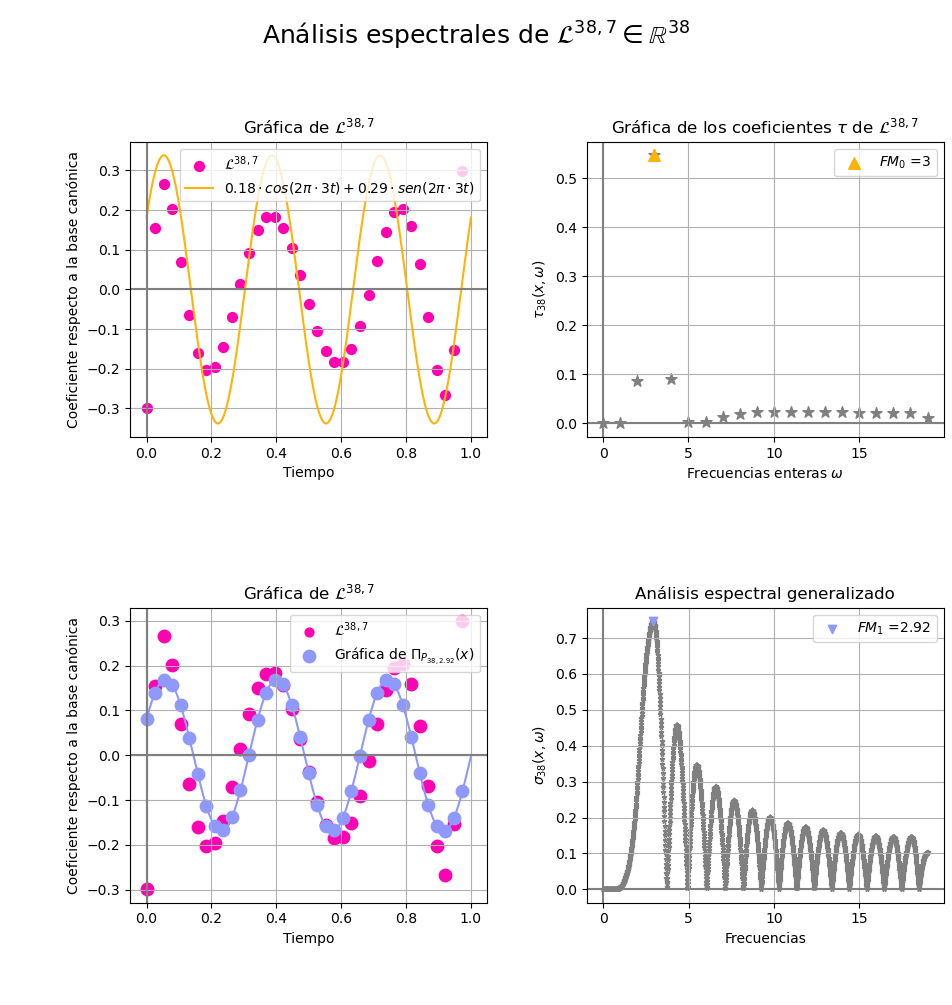
\includegraphics[scale = 0.9]{./estudios_espectrales/ejemplo_pregunta1} 
\end{figure}	

\begin{pregunta}
\label{preg 2}
¿Las frecuencias 
$FP0(\cali{L}^{n,k})$ y $FP1(\cali{L}^{n,k})$
dependen, como implica la pregunta 1, sólo del parámetro
de grado $k$ y no del de dimensión $n$?
Es decir, si $k$, $n_{1}$ y $n_{2}$
son tales que $k \leq n_{1}-1$ y
$k \leq n_{2}-1$, ¿ocurre que 
$FP0(\cali{L}^{n_{1},k})$ = $FP0(\cali{L}^{n_{2},k})$
y 
$FP1(\cali{L}^{n_{1},k})$ = $FP1(\cali{L}^{n_{2},k})$?
\end{pregunta}

Para tratar de responder a la pregunta \ref{preg 2},
fijado un grado $k$,
podría ser útil graficar los puntos de la forma
\begin{equation}
\label{eq0: 8may}
(n, FP0(\cali{L}^{n,k})), \hspace{0.2cm} k < n \leq 69,
\end{equation}
y 
\begin{equation}
\label{eq1: 8may}
(n, FP1(\cali{L}^{n,k})), \hspace{0.2cm} k < n \leq 69.
\end{equation}
Gráficas de este estilo podrían usarse para comprobar
la respuesta a la pregunta \ref{pregunta 1} 
graficando también la recta horizontal $y = \frac{k}{2}$
y viendo si los puntos graficados se encuentran cerca
de esta recta o no. 

\begin{figure}[H]
	\sidecaption{
	 De ser la respuesta
	a la pregunta \ref{preg 2} afirmativa, deberíamos
	de terminar con gráficas de puntos alineados horizontalmente, como
	en este dibujo. Sería bueno que los puntos $FP0$ y $FP1$ estuviesen
	a alturas parecidas, pues eso significaría que los dos análisis espectrales
	dan resultados parecidos.
	\label{fig: ejemplo_pregunta2}
	}
	\centering
	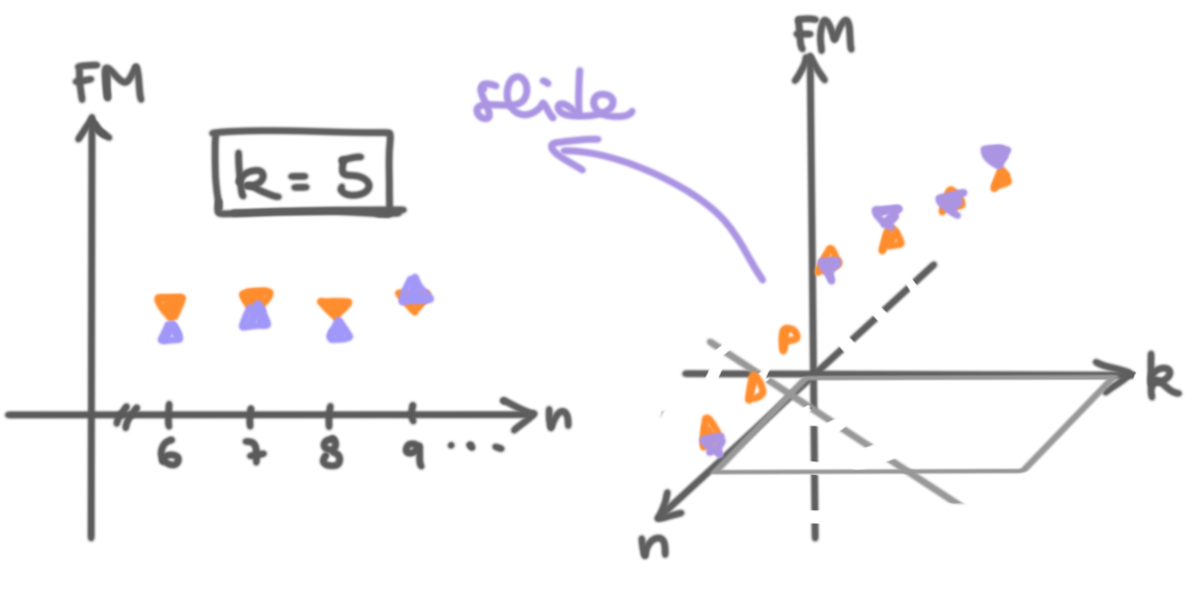
\includegraphics[scale = 1.4]{./estudios_espectrales/ejemplo_pregunta2} 
\end{figure}	


Para intentar refinar la aproximación hecha
en la hipótesis 
\ref{ref: hipotesis}, 
planteemos una tercera y última pregunta. 
Según esta hipótesis,
esperamos que tanto $FP0(\cali{L}^{n,k})$
como $FP1(\cali{L}^{n,k})$ sean cercanos a 
$\frac{k}{2}$; de ocurrir esto, tendríamos que los puntos de
las colecciones 
\begin{equation}
\label{eq5: May1}
(k, FP0(\cali{L}^{n,k})), \hspace{0.2cm} 0 \leq k \leq n-1
\end{equation}
y 
\begin{equation}
\label{eq6: May1}
(k, FP1(\cali{L}^{n,k})), \hspace{0.2cm} 0 \leq k \leq n-1,
\end{equation}
que se obtiene después de hacer análisis espectrales
a todos los PDL de dimensión $n$,
se ajustan a la recta $f(t) = \frac{t}{2}$. 
Una forma de comprobar o refutar esto es calcular las
rectas de mínimos cuadrados de estas dos colecciones
de puntos, y ver si las pendientes de estas son cercanas
a $1/2$ y las ordenadas al origen a $0$.
Planteamos esto en la siguiente


\begin{pregunta}
\label{preg 3}
Fijada una dimensión $2 \leq n \leq 69$,
considere las gráficas de los
puntos \eqref{eq5: May1}
y \eqref{eq6: May1}.

Sean $m_{n,0}$ y $b_{n,0}$ la pendiente y la ordenada
al origen de la recta de mínimos cuadrados calculada a 
partir del conjunto de puntos 
\eqref{eq5: May1}, y
$m_{n,1}$ y $b_{n,1}$ los correspondientes parámetros
para el conjunto de puntos 
\eqref{eq6: May1}.

Considere las nubes de puntos 
\[
(b_{n,0}, m_{n,0}), \hspace{0.2cm} 2 \leq n \leq 69
\]
y 
\[
(b_{n,1}, m_{n,1}), \hspace{0.2cm} 2 \leq n \leq 69.
\]
¿Alrededor de qué punto parecen concentrarse estas nubes?
\end{pregunta}

\begin{figure}[H]
	\sidecaption{
	Se muestran las gráficas 
	de las colecciones de puntos
	\eqref{eq5: May1} y \eqref{eq6: May1}
	para $n=7$	
	descritas en la pregunta
	\ref{preg 3}.
	\label{fig: ejemplo_pregunta3_0}
	}
	\centering
	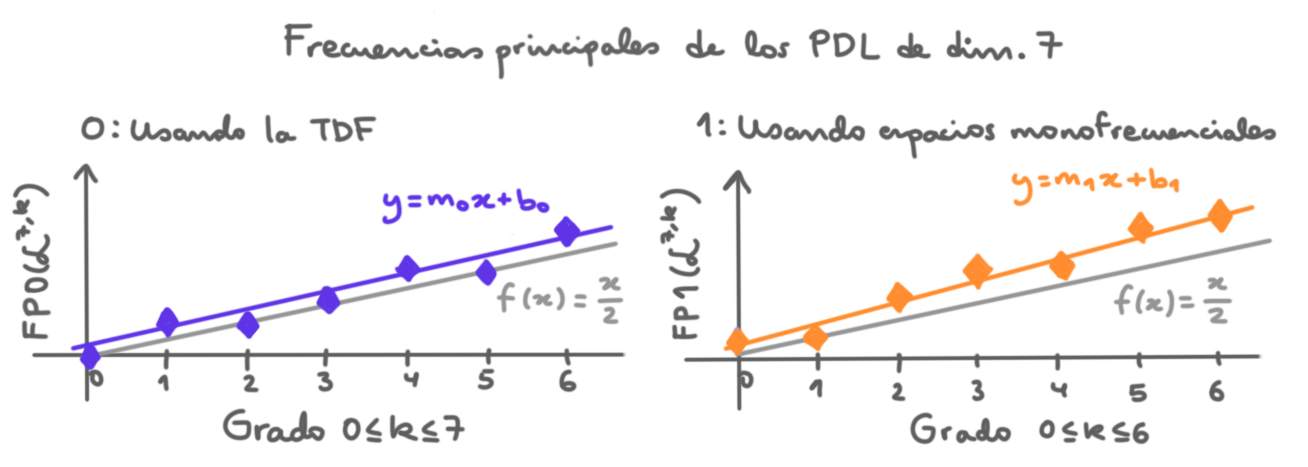
\includegraphics[scale = 1.1]{./estudios_espectrales/ejemplo_pregunta3_0} 
\end{figure}	

\begin{figure}[H]
	\sidecaption{
	Si la estimación dada en la pregunta \ref{pregunta 1} es
	buena, las nubes de puntos descritas en la 
	pregunta \ref{preg 3} deberían estar centradas
	en el punto $(0, 0.5)$.
	\label{fig: ejemplo_pregunta3_1}
	}
	\centering
	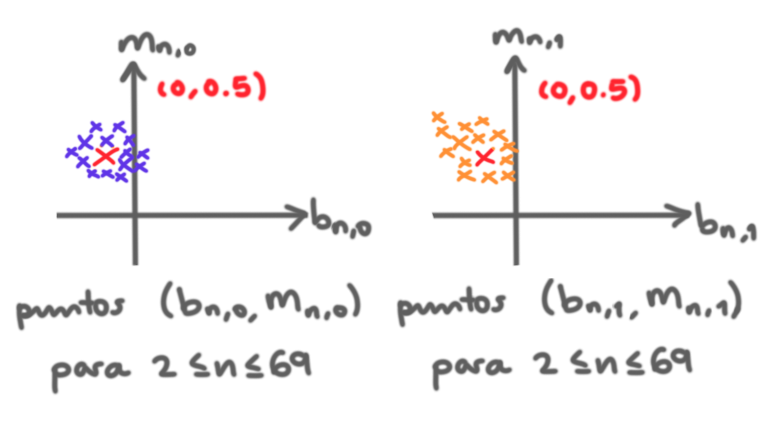
\includegraphics[scale = 1.5]{./estudios_espectrales/ejemplo_pregunta3} 
\end{figure}	


Vamos a responder a estas tres preguntas con gráficas parecidas
a las dibujadas en las figuras
\ref{fig: ejemplo_pregunta1},
\ref{fig: ejemplo_pregunta2},
\ref{fig: ejemplo_pregunta3_0} y
\ref{fig: ejemplo_pregunta3_1}. \\


Intentaremos responder a la pregunta \ref{pregunta 1}
con gráficas análogas
a las expuestas en el ejemplo
\ref{ej: espectros comparacion},
esta vez para analizar algunos PDL; la función con la que
hacemos esto es
\texttt{analisis$\_$espectrales$\_$PDL$\_$mostrarGrafica}. 
Para calcular los datos necesarios para responder
las preguntas \ref{preg 2} y \ref{preg 3},
usando la función \texttt{analisis$\_$espectralPDL$\_$global(n)}
(\TODO{referencia al código del repositorio}), 
para toda dimensión
$2 \leq n \leq 69$ calculamos
\begin{itemize}
	\item los coeficientes $FP1(\cali{L}^{n,k})$ para toda
	$0 \leq k \leq n-1$, y guardamos esta información en el
	array \texttt{sigmasMax$\_$n},
	\item los coeficientes $FP0(\cali{L}^{n,k})$ para toda
	$0 \leq k \leq n-1$, y guardamos esta información en el
	array \texttt{tausMax$\_$n},
	\item y los números $b_{n,0}$, $m_{n,0}$,
	$b_{n,1}$ y $m_{n,1}$ como se definieron en la pregunta
	\ref{preg 3}.
\end{itemize}
Toda esta información se calculó una sola vez y se almacenó
en un diccionario, cuyas llaves son las dimensiones
$n$, y cuyo valor asociado a la llave $n$ es la $6-$tupla
\[
(sigmasMax\_n, tausMax\_n, b_{n,0}, m_{n,0}, b_{n,1}, m_{n,1}).
\]

Usamos el 
módulo \texttt{pickle} para guardar los datos como secuencias
de bytes. El archivo binario en el que se almacenaron los
datos calculados con la función 
\texttt{analisis$\_$espectralPDL$\_$global(n)}
es \texttt{data$\_$AE.txt}. \\

La función con la que obtenemos gráficas análogas 
a la de la figura 
\ref{fig: ejemplo_pregunta2} es
\texttt{grafica$\_$analisisGlobal$\_$k$\_$fijo}
y, para obtener gráficas análogas a la de la figura
\ref{fig: ejemplo_pregunta3_0},
usamos \texttt{graficar$\_$analisis$\_$espectralPDL$\_$global}.

Recordamos que,
para cada análisis espectral,
vamos a tomar al conjunto de 
frecuencias 
como se sugiere en la nota \ref{nota: muestreo dom frecuencia}.

\section{Gráficas y comentarios}
Las gráficas de los espectros
para los PDL de dimensión hasta $40$, así
como gráficas análogas a las de las figuras
\ref{fig: ejemplo_pregunta2}
y 
\ref{fig: ejemplo_pregunta3}
se han guardado en \TODO{cita la carpeta del
repositorio
con las imágenes.}
A continuación, mostramos algunas
de estas imágenes con algunos comentarios
que nos ayuden a responder numéricamente a 
las preguntas
\ref{pregunta 1}, \ref{preg 2} y \ref{preg 3}
planteadas antes. \\

Veamos qué pasa con $n=7$.

\begin{figure}[H]
	\sidecaption{
	\label{fig: 7_0}
	}
	\centering
	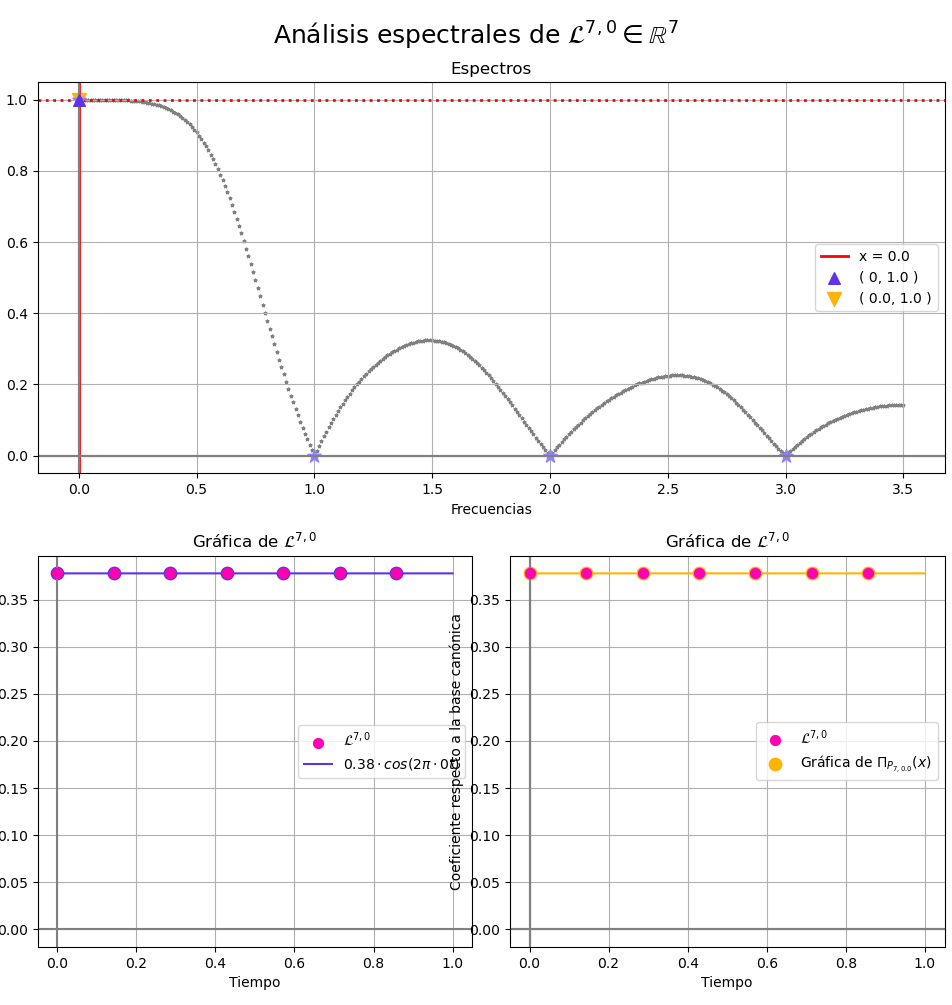
\includegraphics[scale = 0.3]{./graficas_analisisEspectrales/7_0} 
\end{figure}	

\begin{figure}[H]
	\sidecaption{
	\label{fig: 7_1}
	}
	\centering
	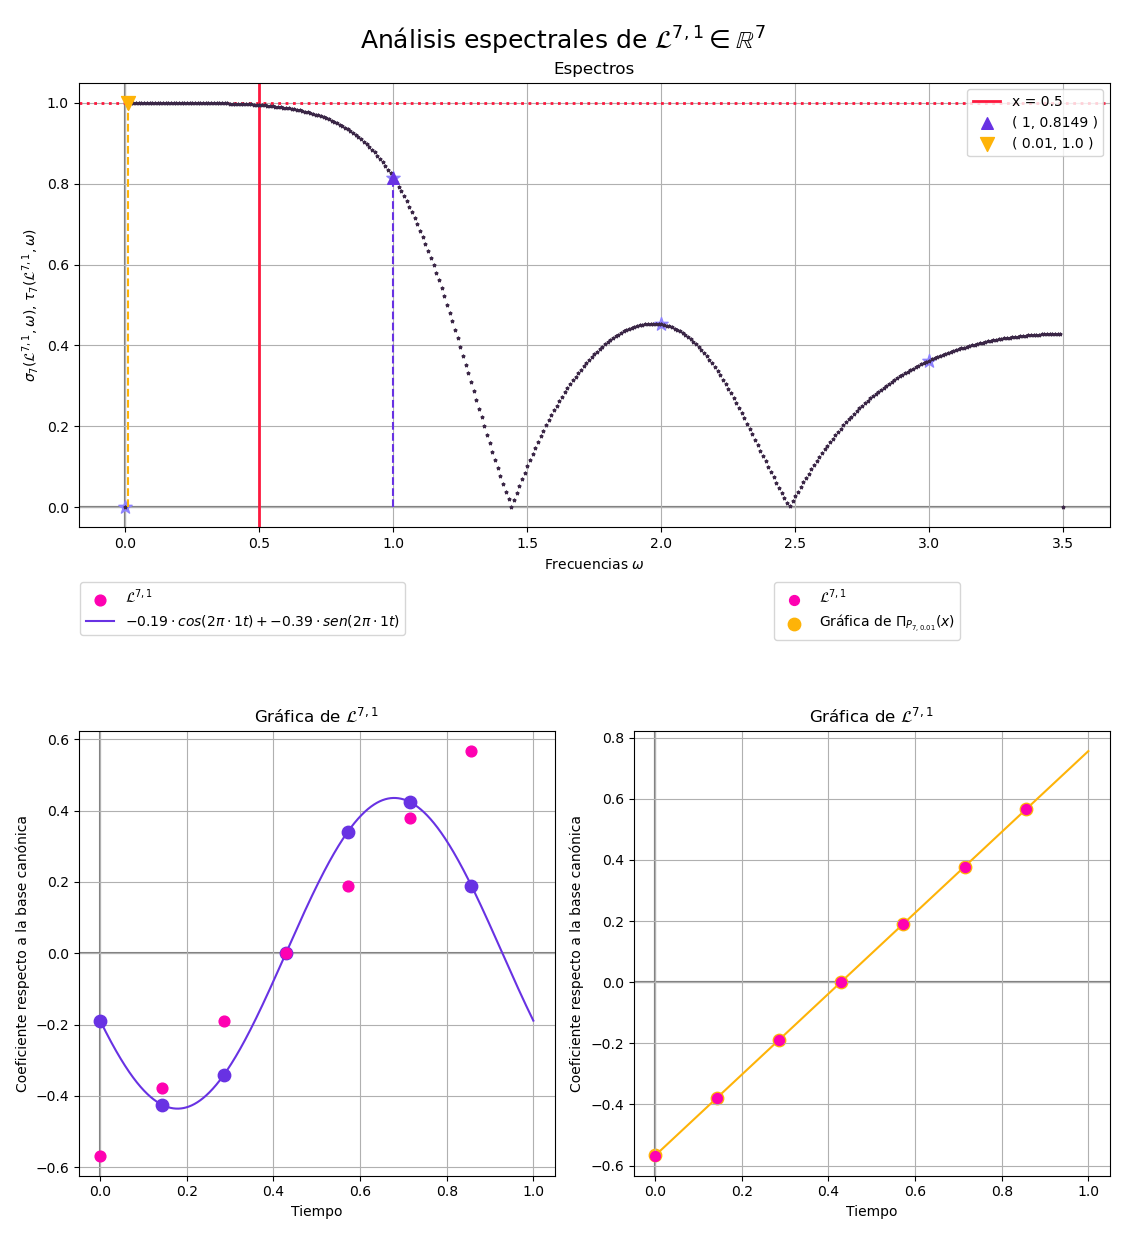
\includegraphics[scale = 0.3]{./graficas_analisisEspectrales/7_1} 
\end{figure}	

\begin{figure}[H]
	\sidecaption{
	\label{fig: 7_2}
	}
	\centering
	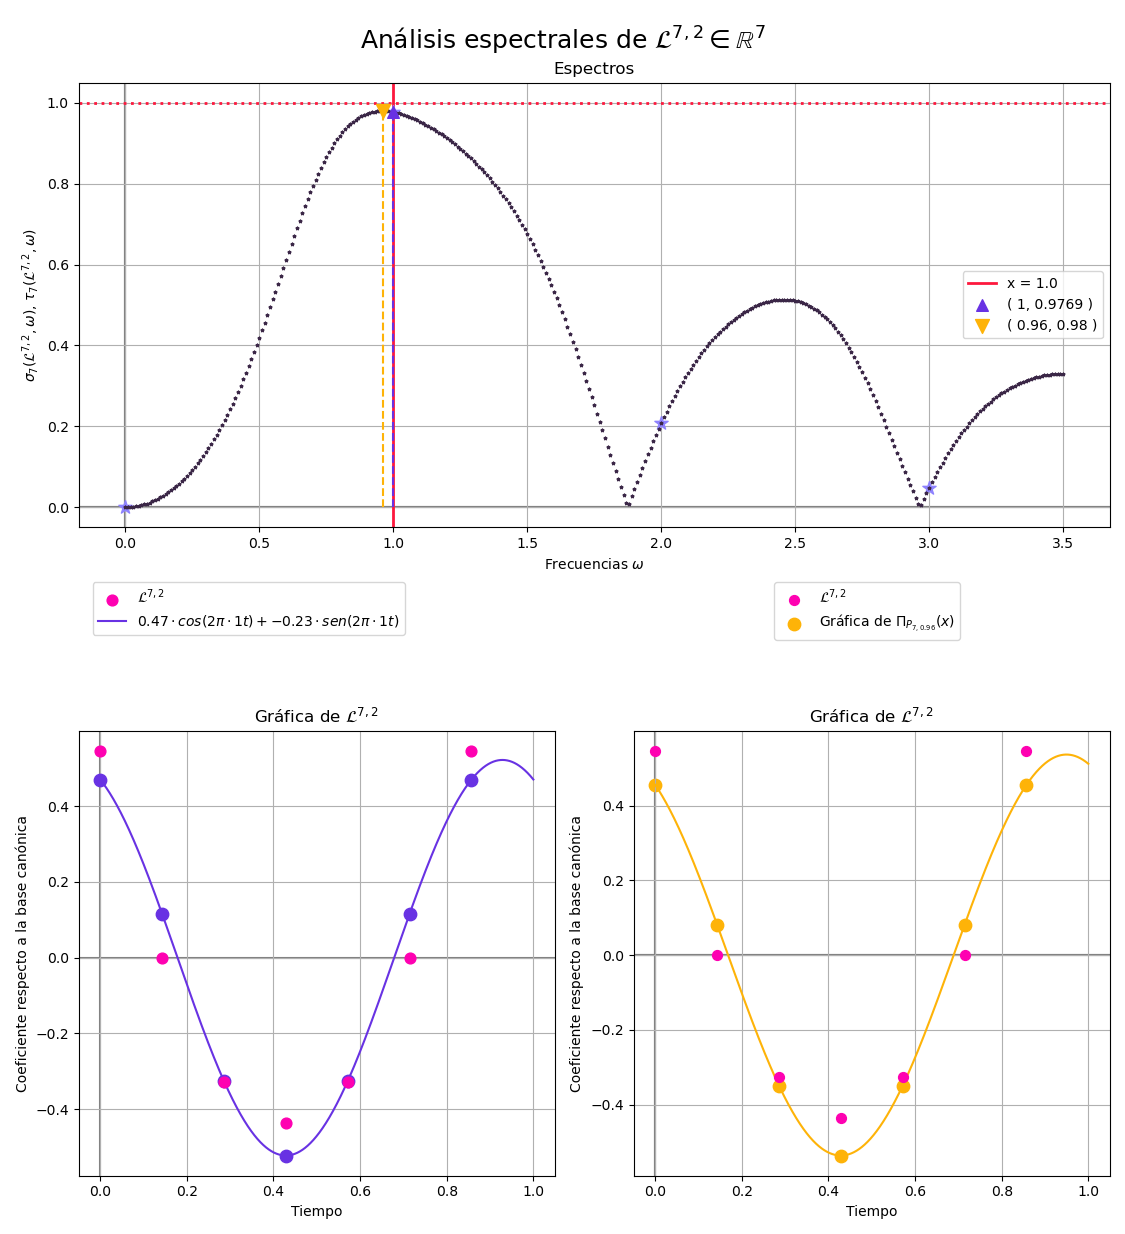
\includegraphics[scale = 0.3]{./graficas_analisisEspectrales/7_2} 
\end{figure}	


\begin{figure}[H]
	\sidecaption{
	\label{fig: 7_3}
	}
	\centering
	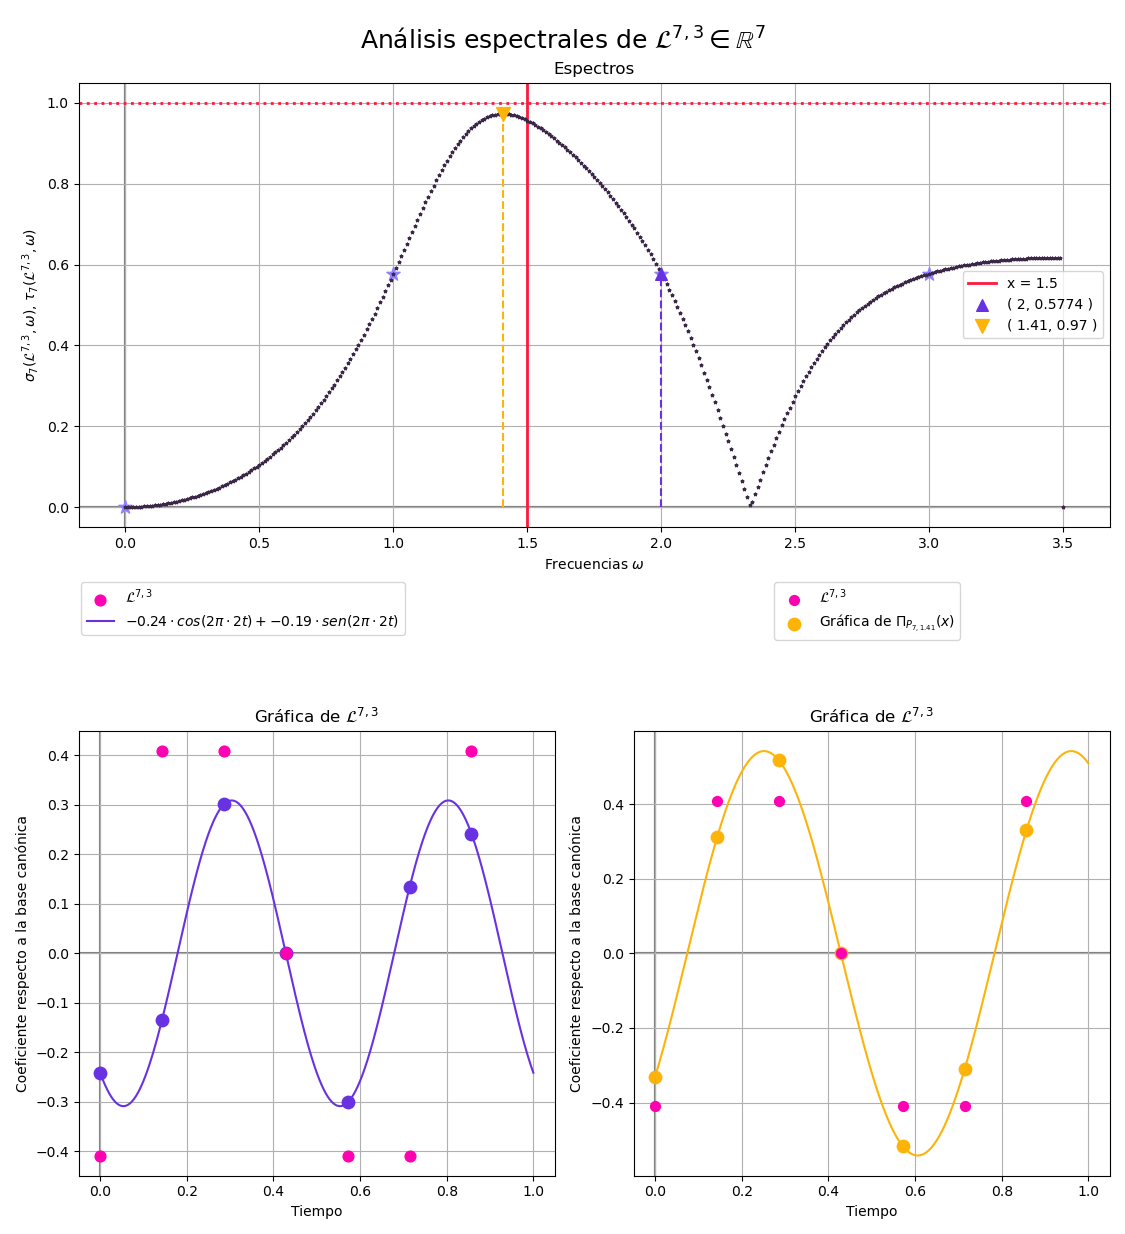
\includegraphics[scale = 0.3]{./graficas_analisisEspectrales/7_3} 
\end{figure}	


\begin{figure}[H]
	\sidecaption{
	\label{fig: 7_4}
	}
	\centering
	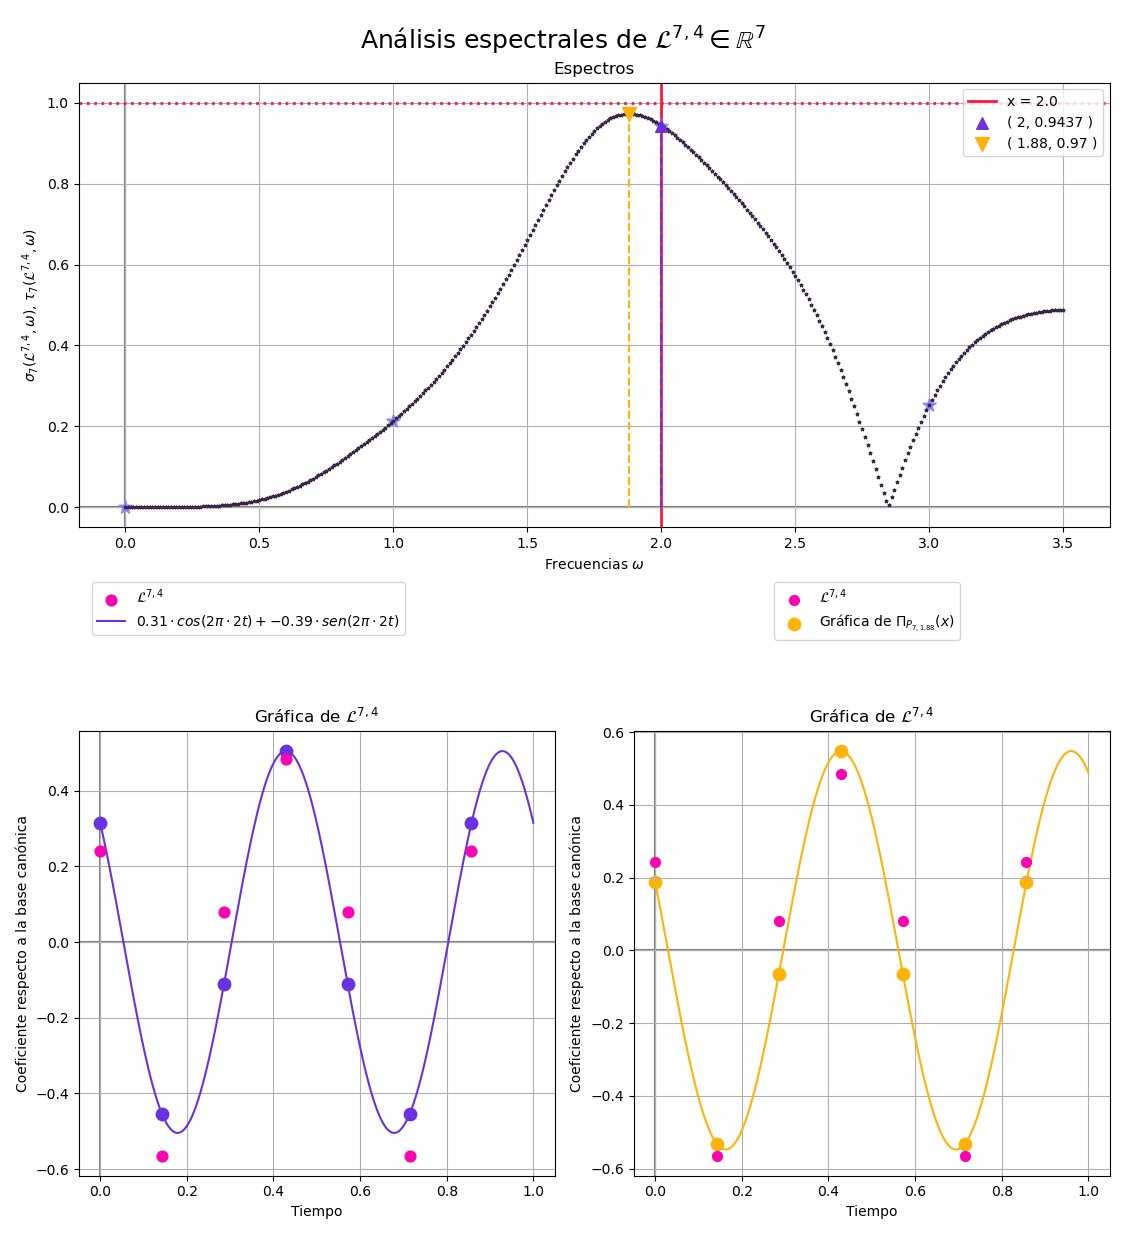
\includegraphics[scale = 0.3]{./graficas_analisisEspectrales/7_4} 
\end{figure}	


\begin{figure}[H]
	\sidecaption{
	\label{fig: 7_5}
	}
	\centering
	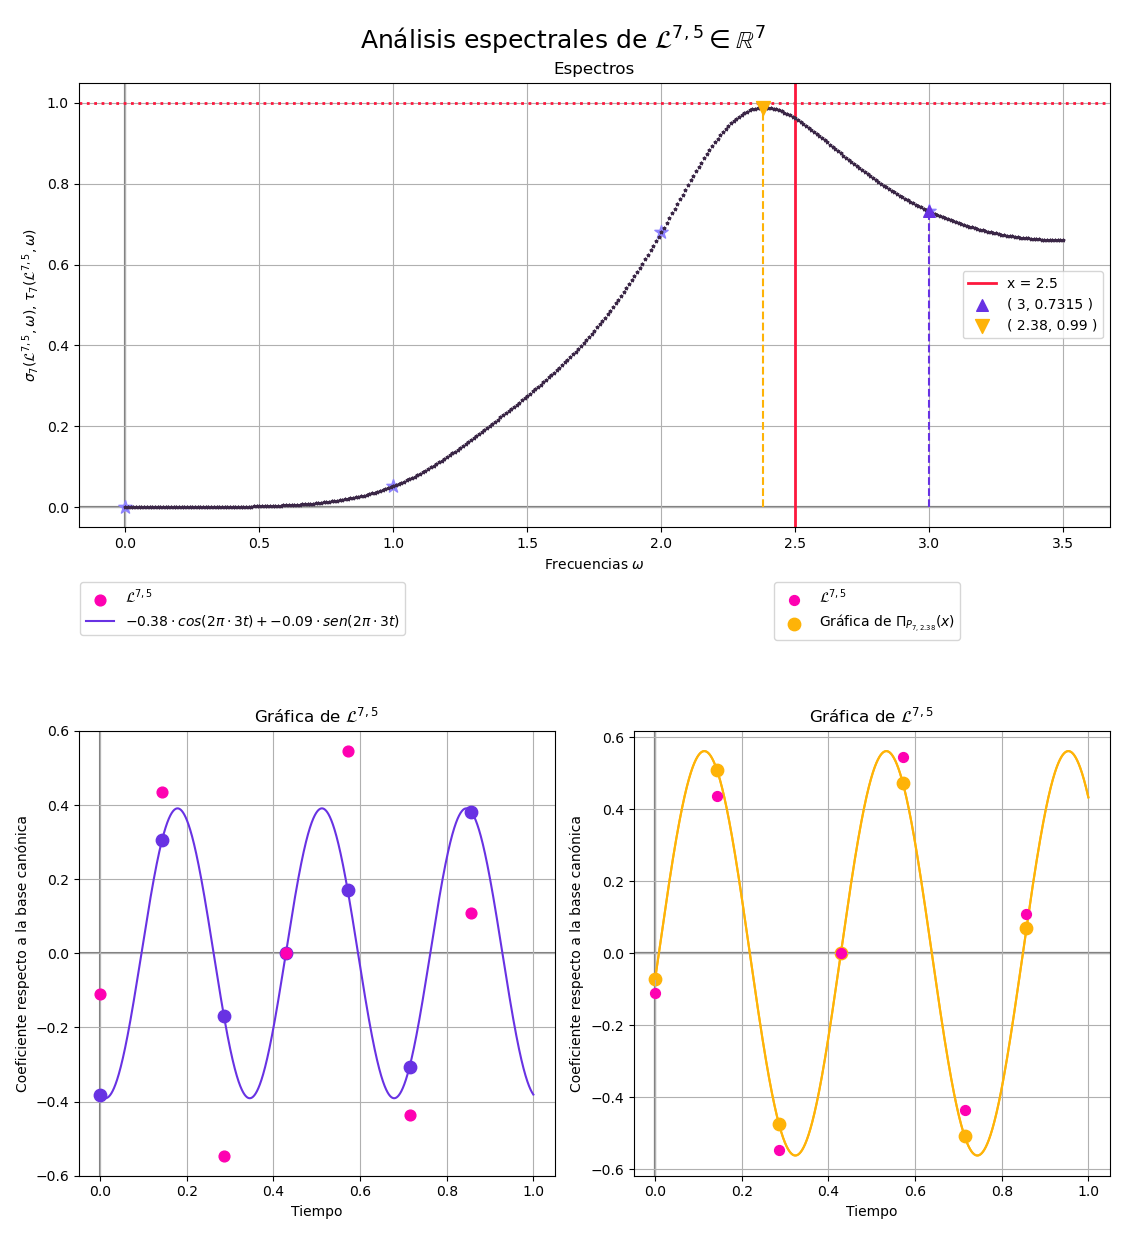
\includegraphics[scale = 0.3]{./graficas_analisisEspectrales/7_5} 
\end{figure}	


\begin{figure}[H]
	\sidecaption{
	\label{fig: 7_6}
	}
	\centering
	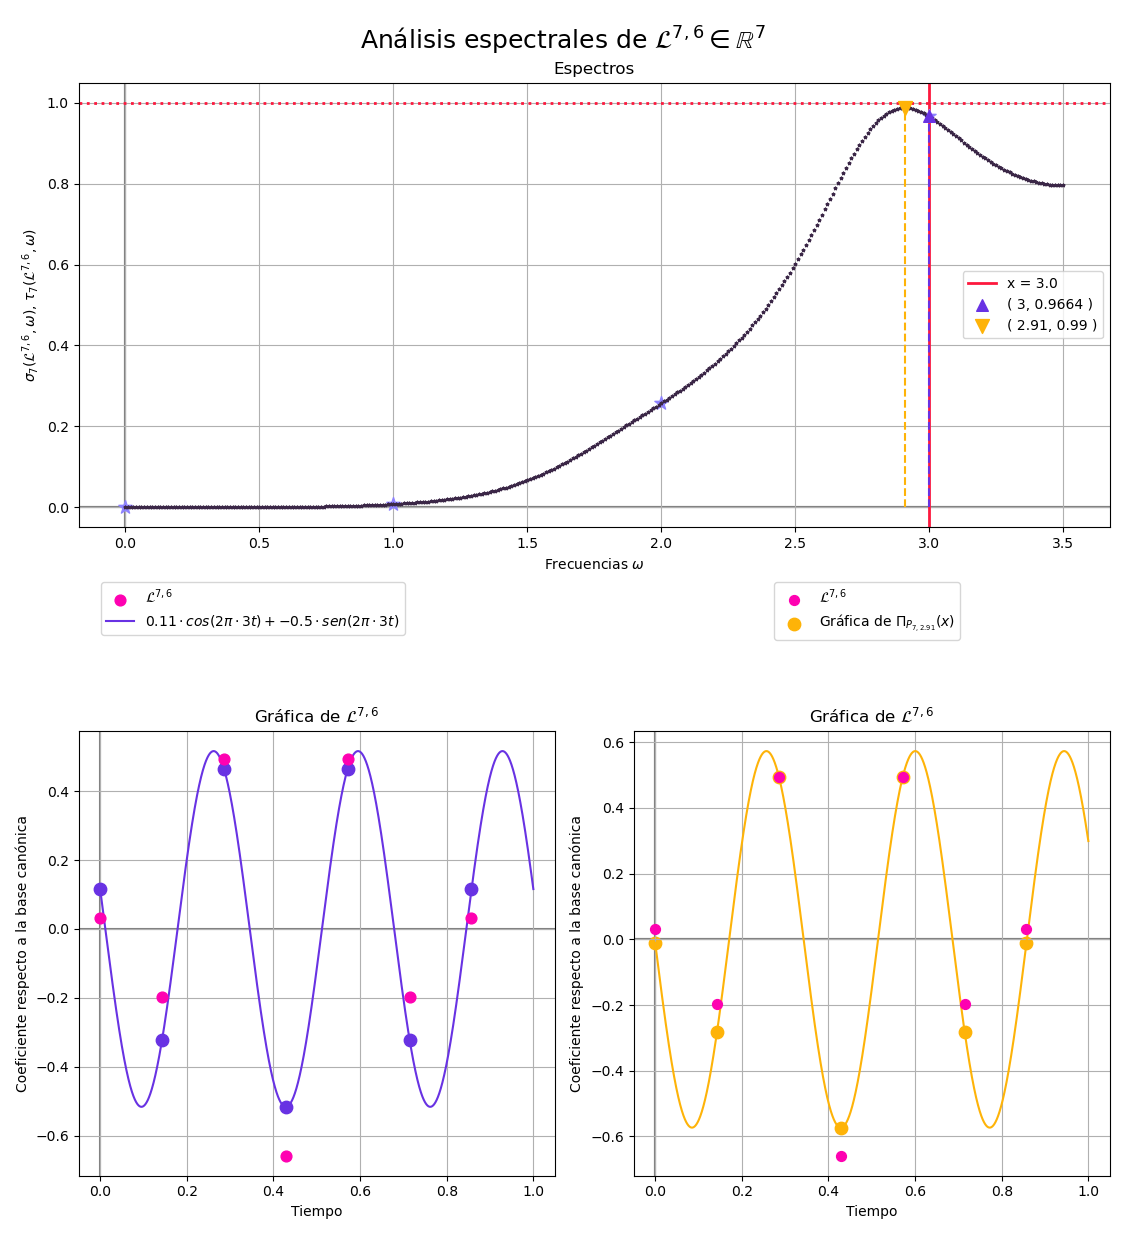
\includegraphics[scale = 0.3]{./graficas_analisisEspectrales/7_6} 
\end{figure}	

A continuación mostramos las gráficas de los puntos
de la forma $(k, FP0(\cali{L}^{7,k}))$
y $(k, FP0(\cali{L}^{7,k}))$.
\begin{figure}[H]
	\sidecaption{
	Observe que $FP0(\cali{L}^{7,0}) = 0 = FP1(\cali{L}^{7,0})$
	pero $FP0(\cali{L}^{7,1}) = 1 $ mientras que 
	$FP1(\cali{L}^{7,1})$, aunque no es cero, es un decimal muy cercano
	a cero; observe en la figura \ref{fig: 7_0,1}, donde se dibujan
	los espectros de los dos primeros PDL de dimensión $7$ que, en efecto,
	usando un sinusoide de frecuencia 
	$0.01$ (la dada por el espectro
	basado en espacios monofrecuenciales), 
	logramos ajustar casi a la perfección la gráfica de $\cali{L}^{7,1}$
	(que, según el teorema \ref{cor: BON de legendre para espacios Wk}, yace
	en una recta, por lo que no puede ser ajustada a la perfección por un
	sinusoide),
	mientras que usando un sinusoide de frecuencia $1$ (la dada por el 
	espectro basado en la TDF), no se logran ajustar tan bien los datos.
	\label{fig: 7}
	}
	\centering
	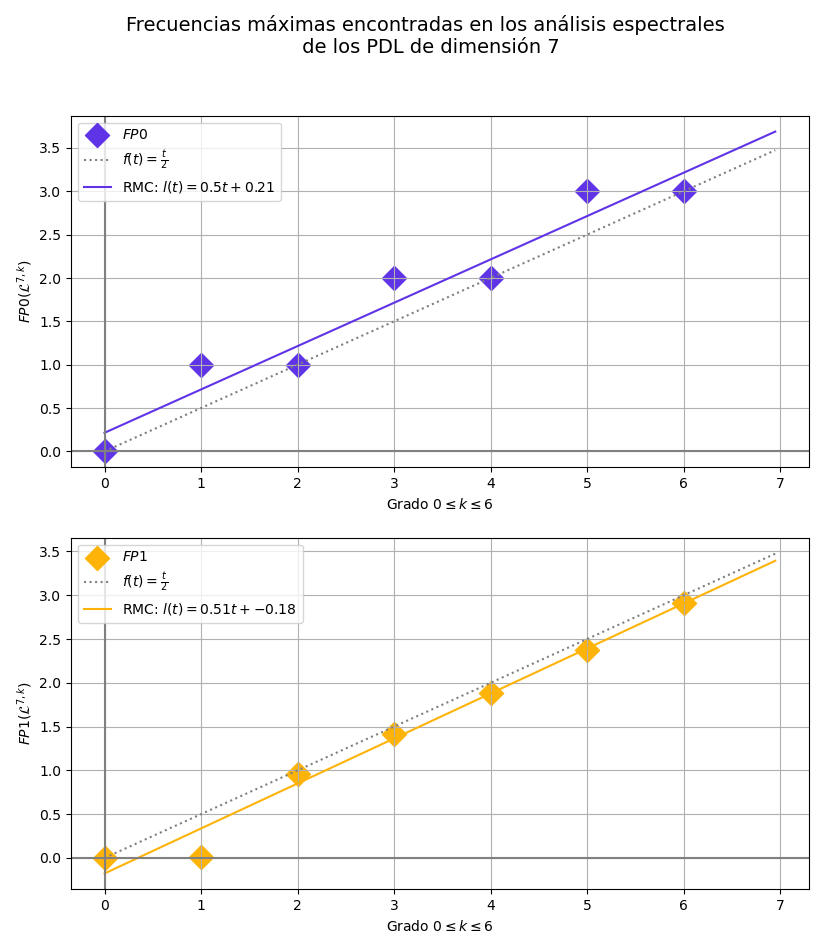
\includegraphics[scale = 0.5]{./estudios_espectrales/7} 
\end{figure}	

Como notamos en la descripción de la figura
\ref{fig: 7}, parece ser que usando el estudio espectral basado en 
espacios monofrecuenciales obtenemos una aproximación de la gráfica
de $\cali{L}^{n,1}$, con $n=7$, en base a un sinusoide de frecuencia muy baja;
grafiquemos 
los puntos de la forma
\eqref{eq0: 8may} y \eqref{eq1: 8may} para 
$k=1$
para ver si esta es una particularidad de la dimensión
$n=7$ o si también ocurre para otros valores de $n$.

\begin{figure}[H]
	\sidecaption{
	Comprobamos numéricamente que los resultados del espectro-1
	sugieren usar frecuencias muy bajas para modelar los 
	PDL de grado $1$; la única excepción se da para $n=3$. Graficamos
	a continuación los espectros de $\cali{L}^{3,1}$ para ver qué
	está sucediendo.
	\label{fig: k_1}
	}
	\centering
	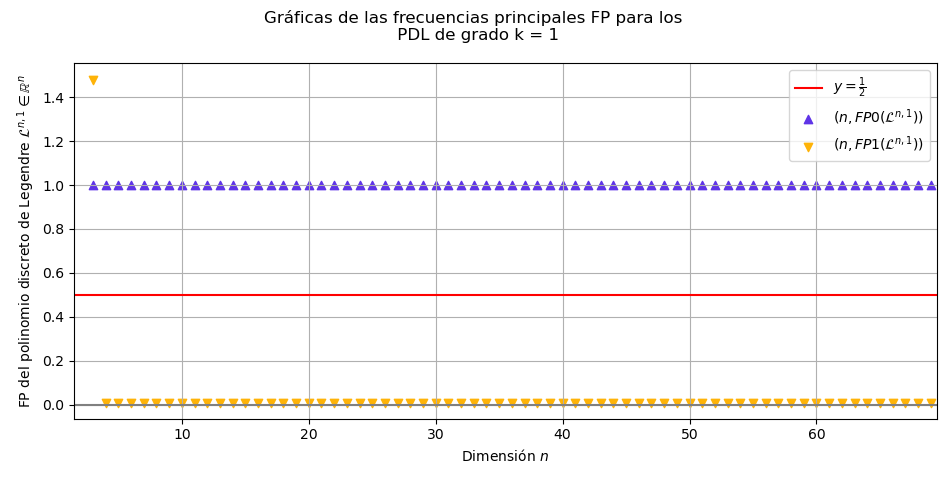
\includegraphics[scale = 0.5]{./estudios_espectrales/k_1} 
\end{figure}	


\begin{figure}[H]
	\sidecaption{
	Como se muestra en los espectros, el coeficiente
	$\sigma_{3}(\mathcal{L}^{3,1}, \omega)$ es, para casi toda
	$\omega$ considerada, muy cercana a uno, por lo que cualquiera
	de estas frecuencias sería adecuada para aproximar con un sinusoide la 
	gráfica de $\mathcal{L}^{3,1}$. Por la forma en que programamos
	el proceso, se usa la última frecuencia más alta, que resultó ser
	$1.48$. Como puede comprobar en las gráficas de abajo, se puede
	aproximar bien la gráfica de $\mathcal{L}^{3,1}$ tanto
	con frecuencia $\omega = 1$ como con frecuencia
	$\omega = 1.48$.
	\label{fig: 3_1}
	}
	\centering
	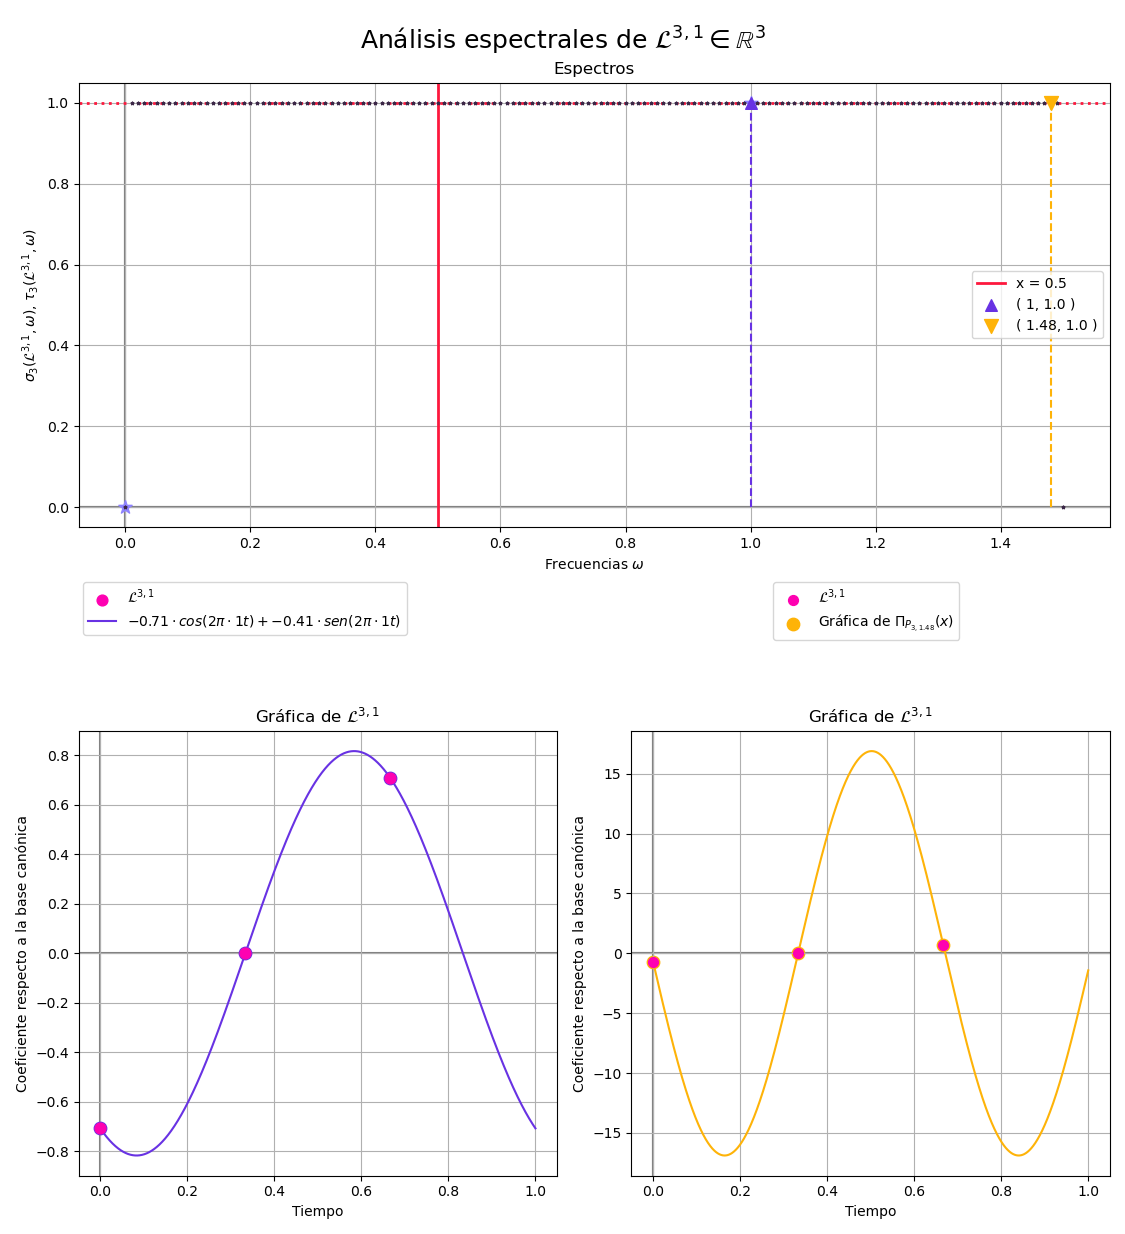
\includegraphics[scale = 0.45]{./estudios_espectrales/3_1} 
\end{figure}	

Comprobemos, graficando los espectros 
de algunos PDL de grado $1$ y dimensión mayor a $3$, 
que frecuencias muy cercanas a $0$ son buenas para modelar
la gráfica de $\cali{L}^{n,1}$, hecho que es 
sugerido por la figura \ref{fig: k_1}.

\begin{figure}[H]
	\sidecaption{
	Note que en este espectro no ocurre lo que se tenía
	en el del PDL $\cali{L}^{3,1}$ (c.f. figura 
	\ref{fig: 3_1}); en este caso, el espectro-$1$ muestra
	claramente que $\omega =0.1$, la frecuencia en $Dom_{\omega, n}$
	más cercana a $0$ que \textbf{no} es cero, es la mejor
	(c.f. nota 
	\ref{nota: la mejor frecuencia}).
	\label{fig: 8_1}
	}
	\centering
	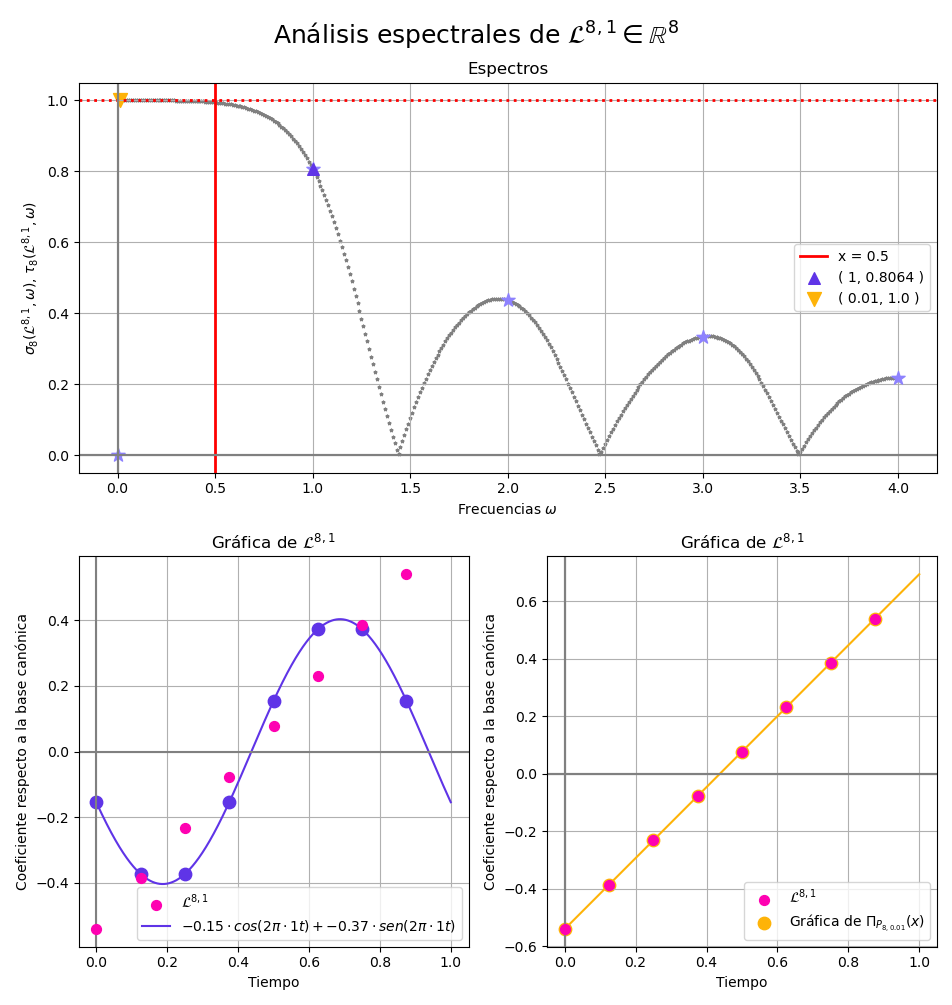
\includegraphics[scale = 0.45]{./estudios_espectrales/8_1} 
\end{figure}	

\begin{figure}[H]
	\sidecaption{
	}
	\centering
	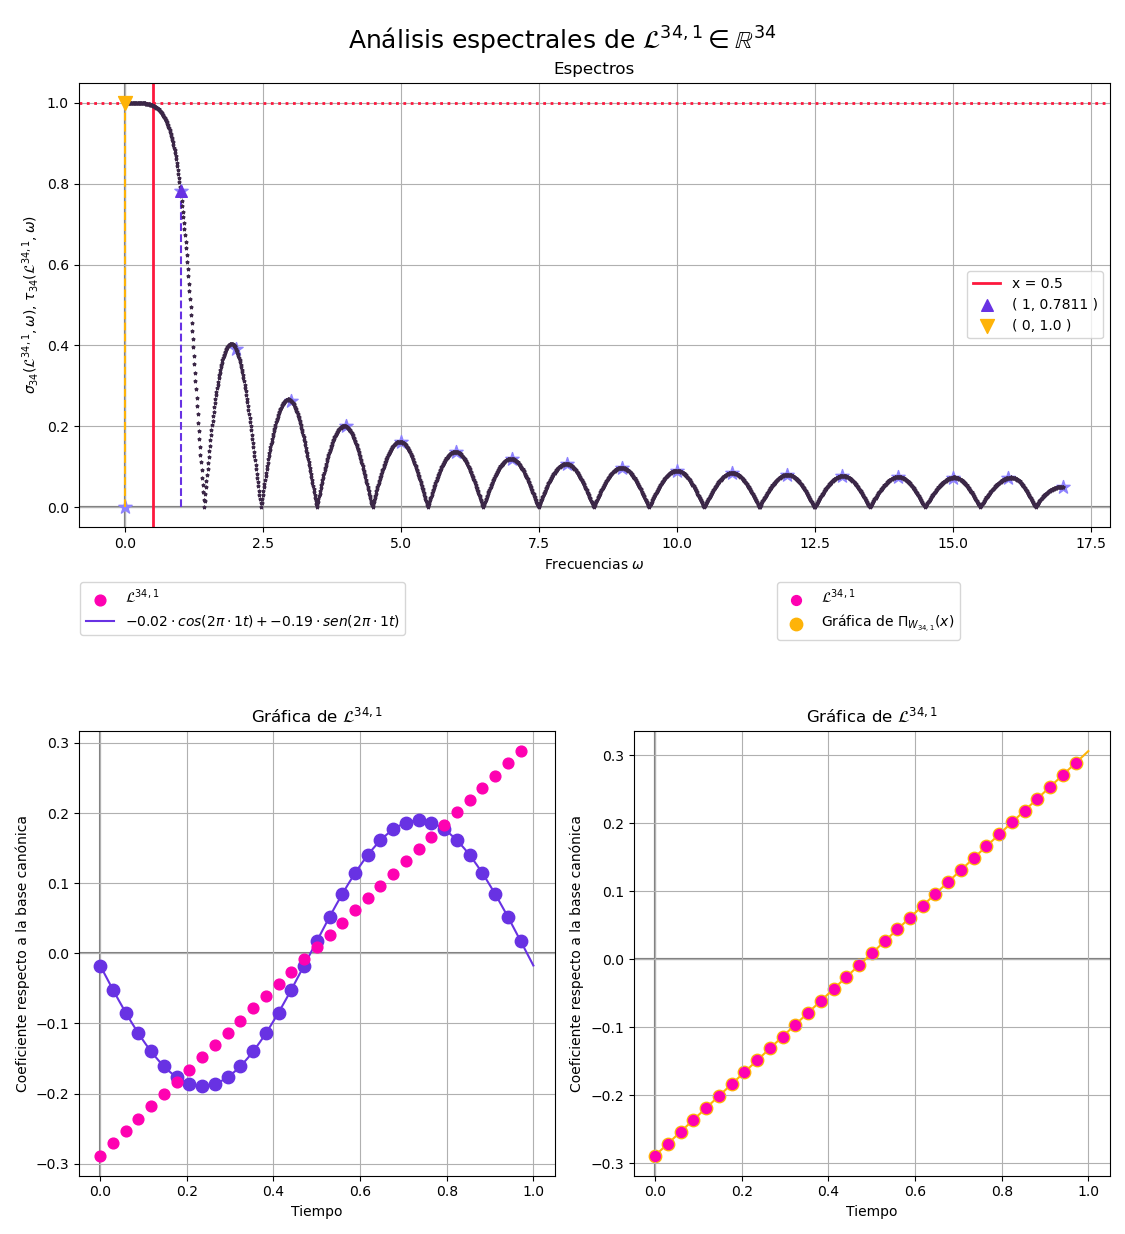
\includegraphics[scale = 0.45]{./estudios_espectrales/34_1} 
\end{figure}	

Graficando algunos PDL de dimensión
39, apreciamos que conforme $k$ aumenta, es menos
sencillo aproximar la gráfica del respectivo PDL
con un sinusoide.
\begin{figure}[H]
	\sidecaption{
	}
	\centering
	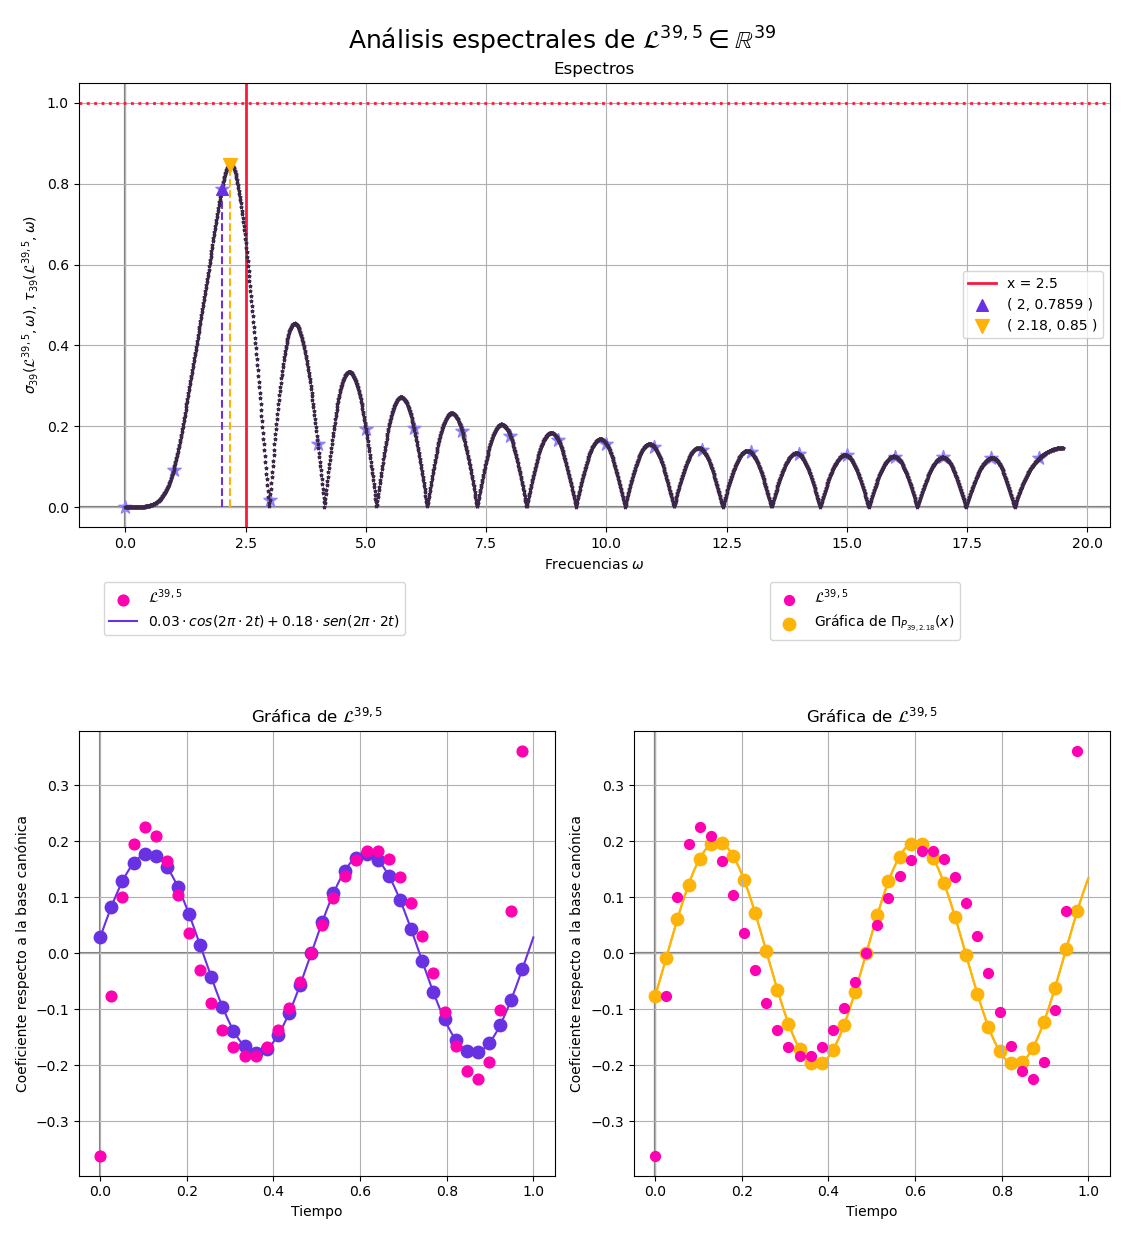
\includegraphics[scale = 0.45]{./estudios_espectrales/39_5} 
\end{figure}	
\begin{figure}[H]
	\sidecaption{
	}
	\centering
	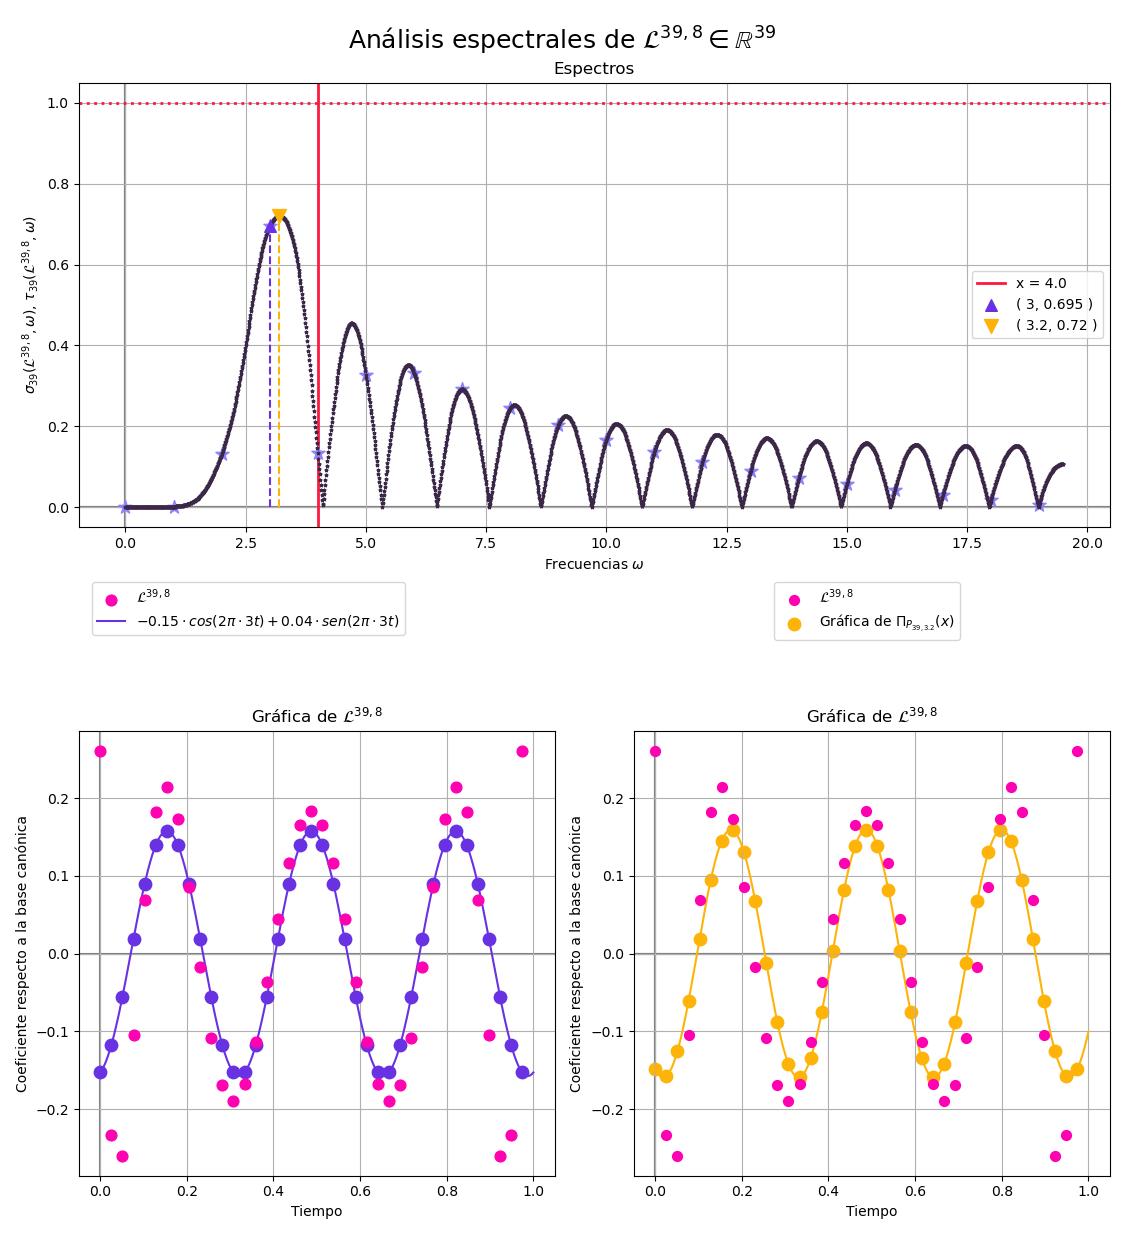
\includegraphics[scale = 0.45]{./estudios_espectrales/39_8} 
\end{figure}	
\begin{figure}[H]
	\sidecaption{
	}
	\centering
	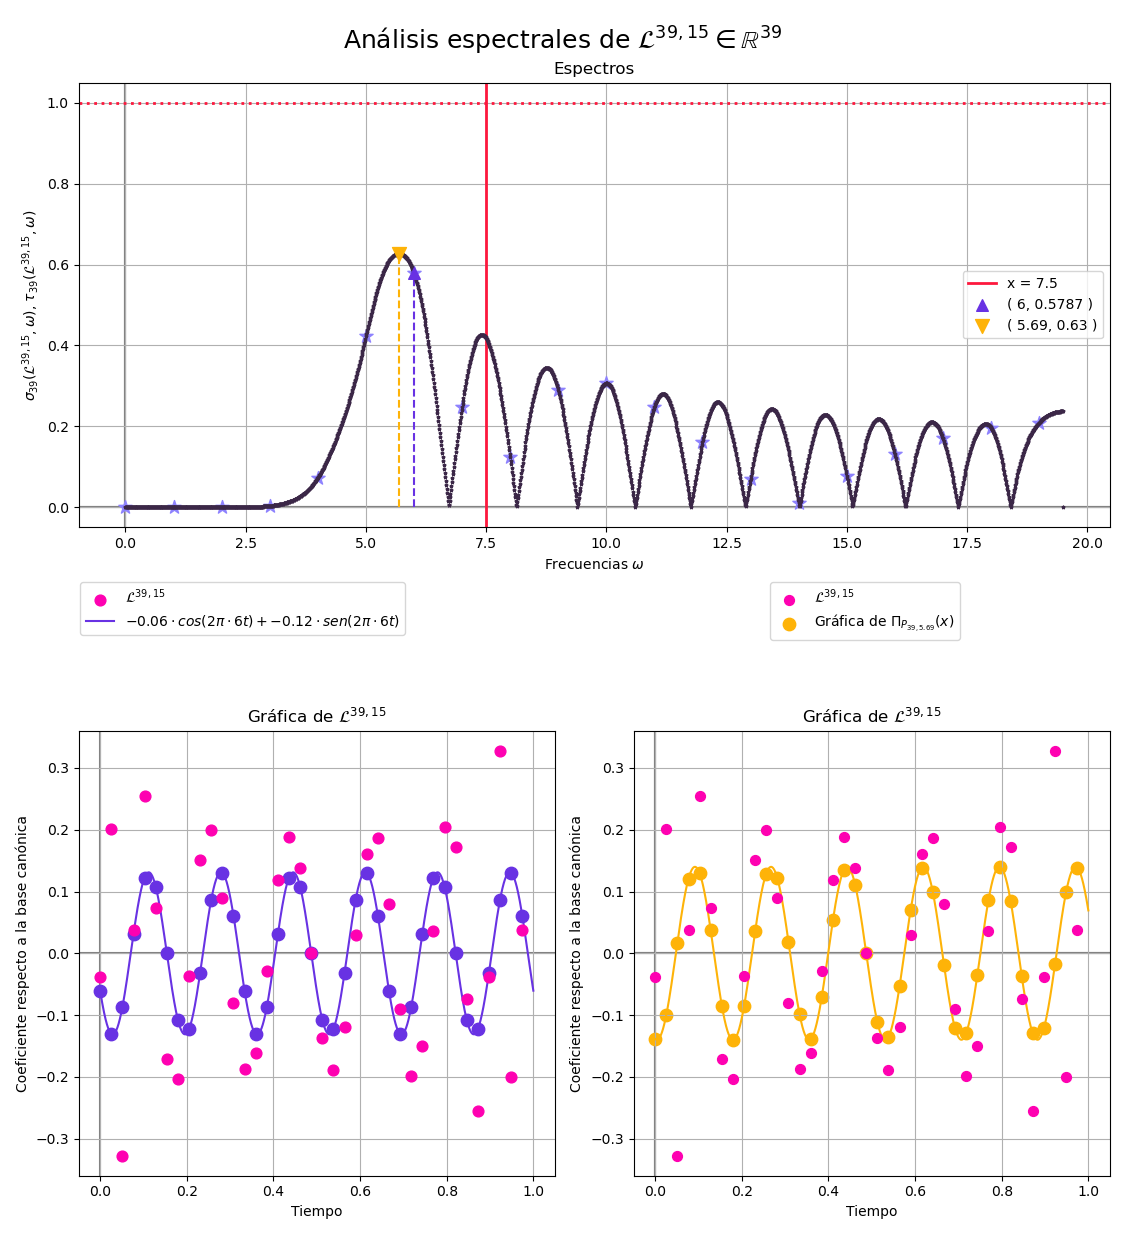
\includegraphics[scale = 0.45]{./estudios_espectrales/39_15} 
\end{figure}	
\begin{figure}[H]
	\sidecaption{
	}
	\centering
	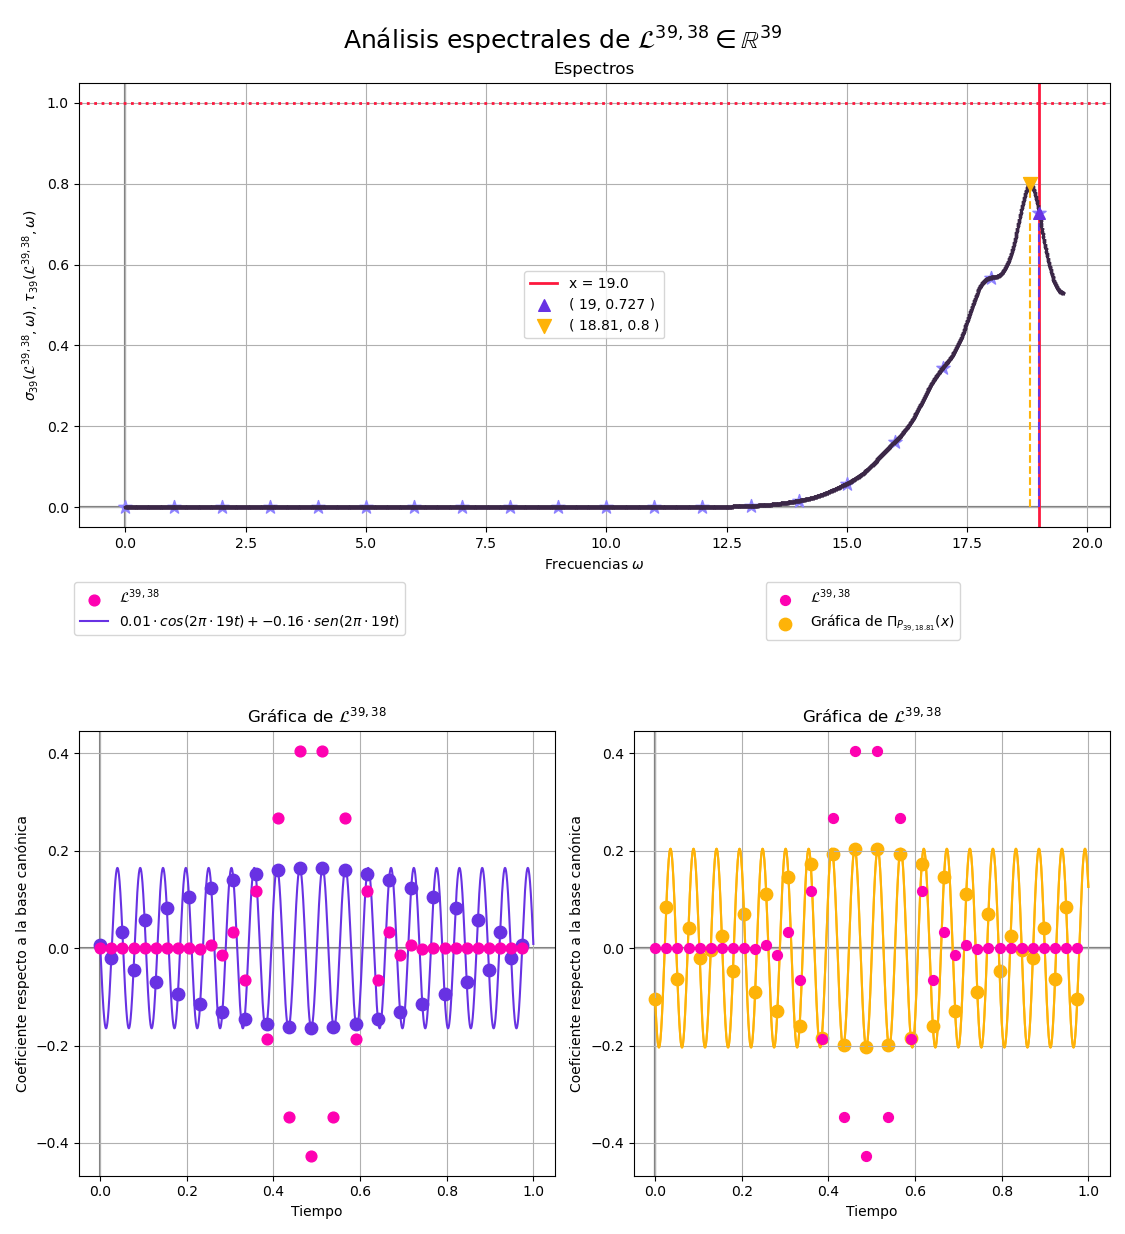
\includegraphics[scale = 0.3]{./estudios_espectrales/39_38} 
\end{figure}	
\begin{figure}[H]
	\sidecaption{
	}
	\centering
	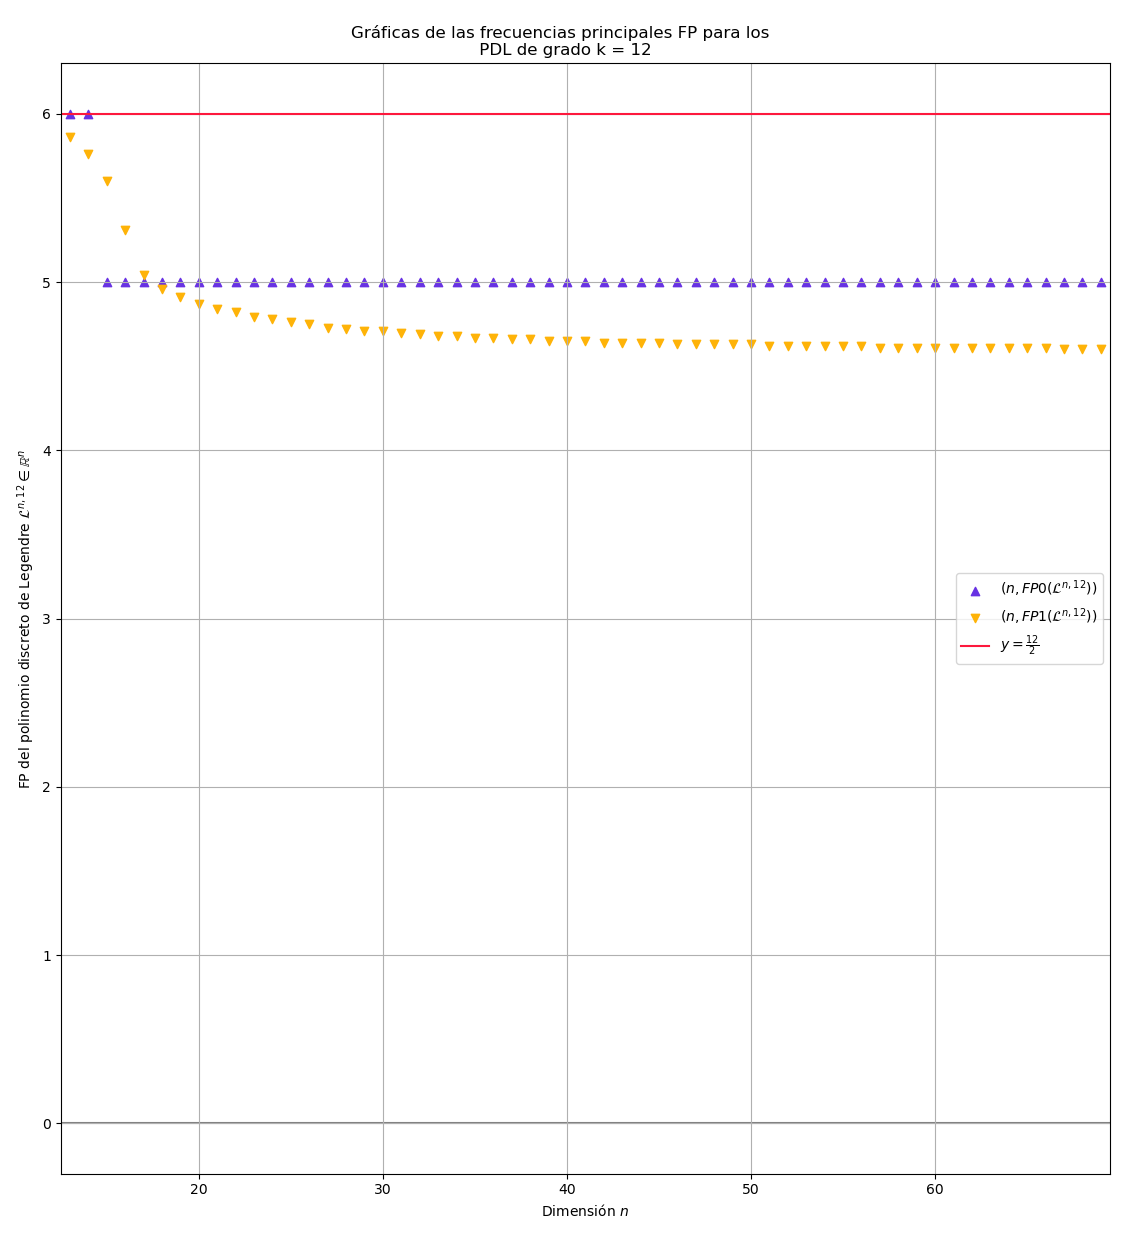
\includegraphics[scale = 0.3]{./estudios_espectrales/k_12} 
\end{figure}	
\begin{figure}[H]
	\sidecaption{
	}
	\centering
	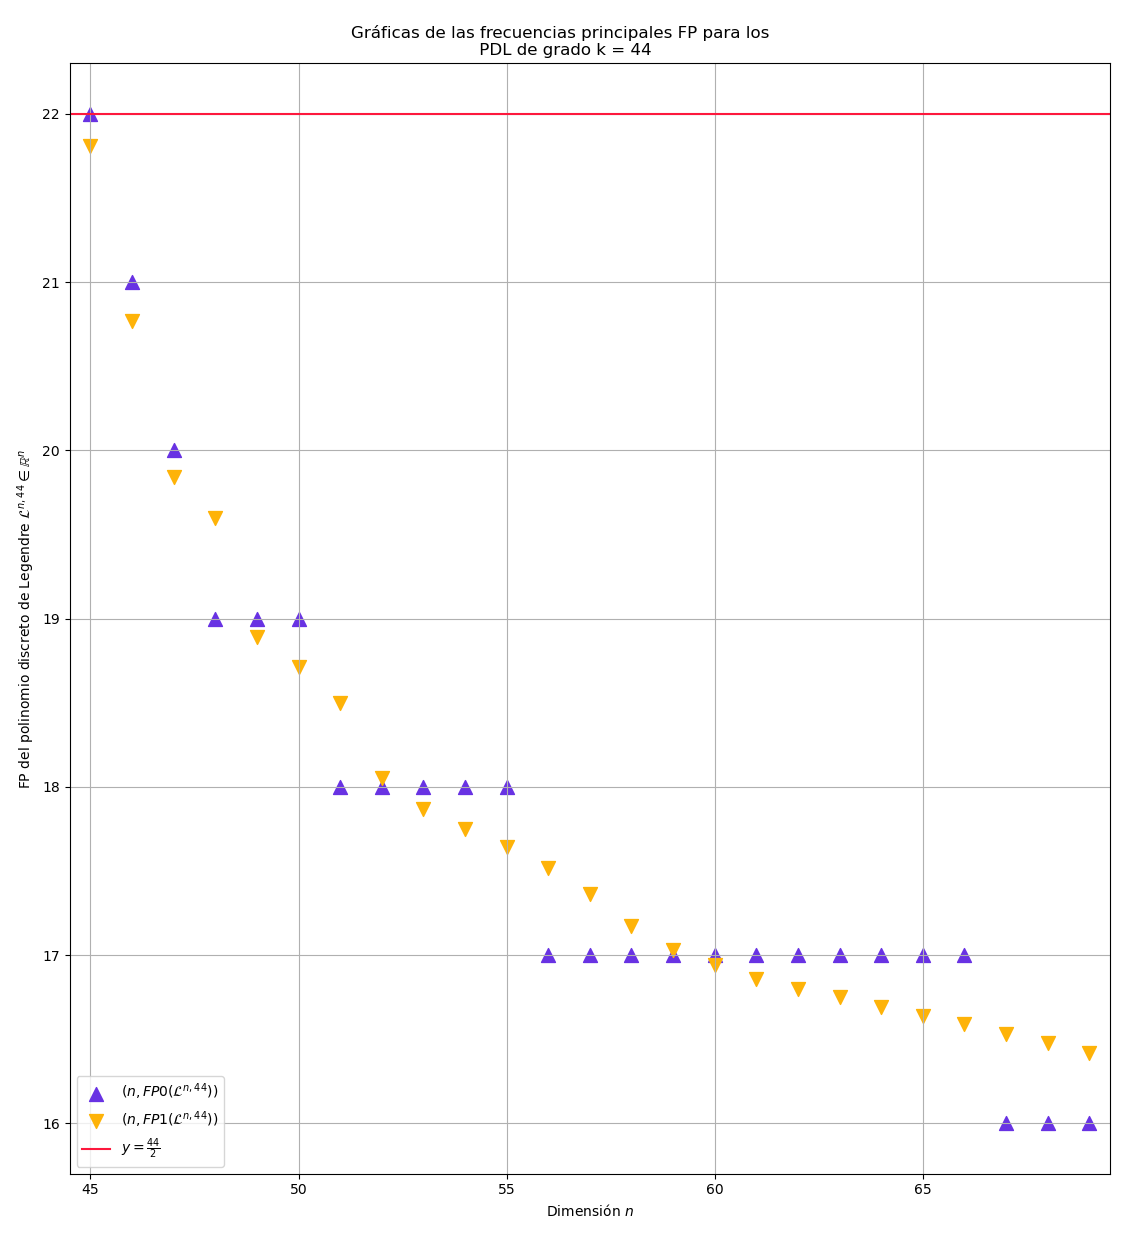
\includegraphics[scale = 0.3]{./estudios_espectrales/k_44} 
\end{figure}	
\begin{figure}[H]
	\sidecaption{
	}
	\centering
	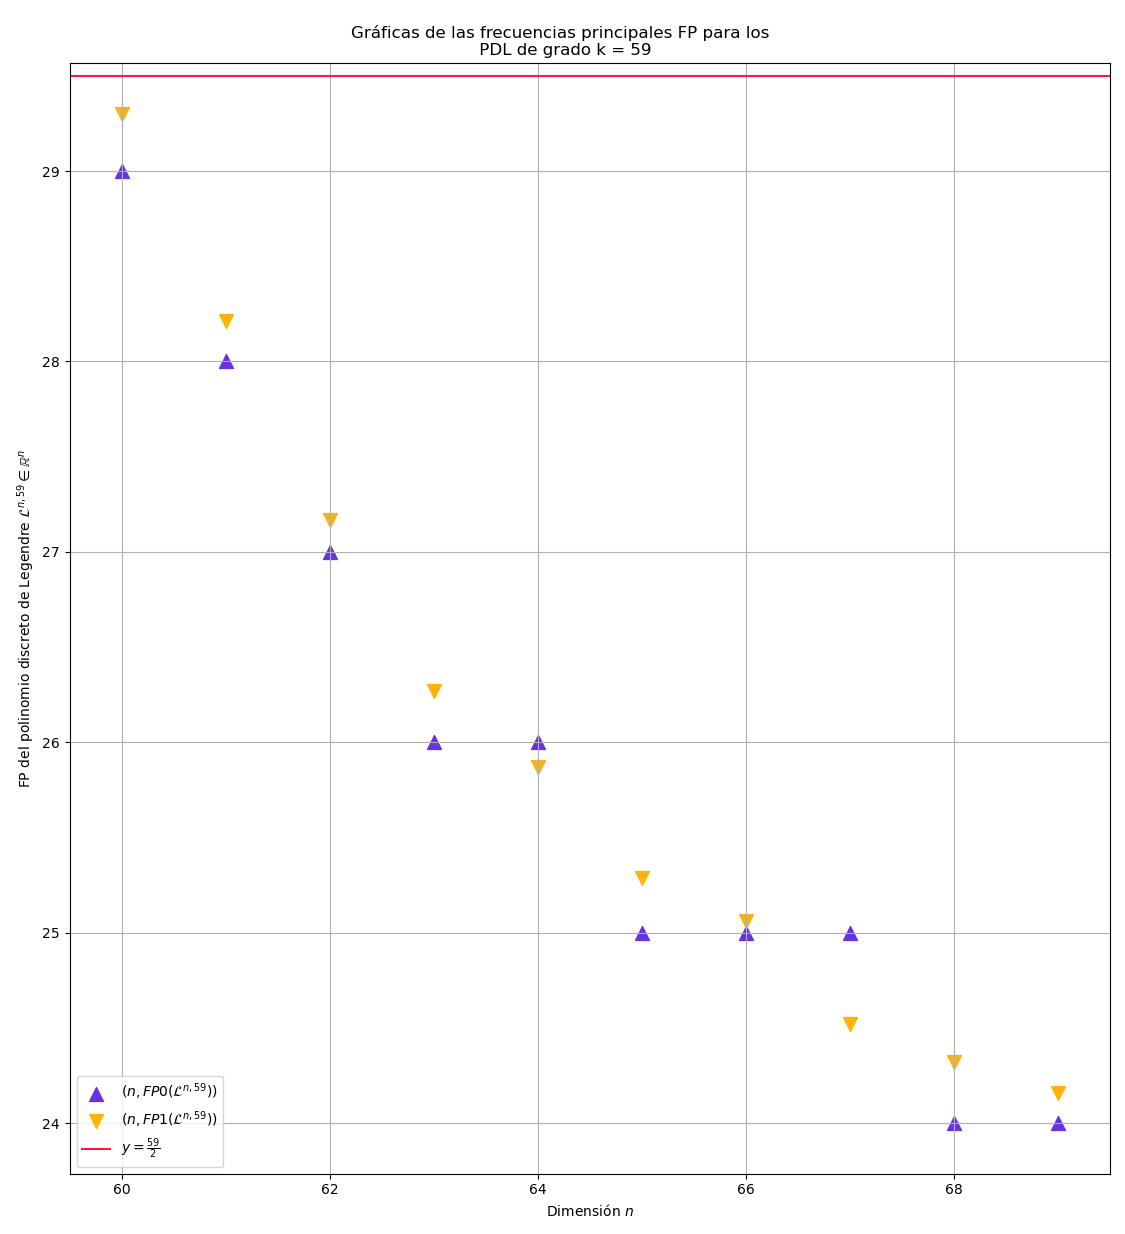
\includegraphics[scale = 0.3]{./estudios_espectrales/k_59} 
\end{figure}	


\begin{figure}[H]
	\sidecaption{
	\label{fig: 30}
	}
	\centering
	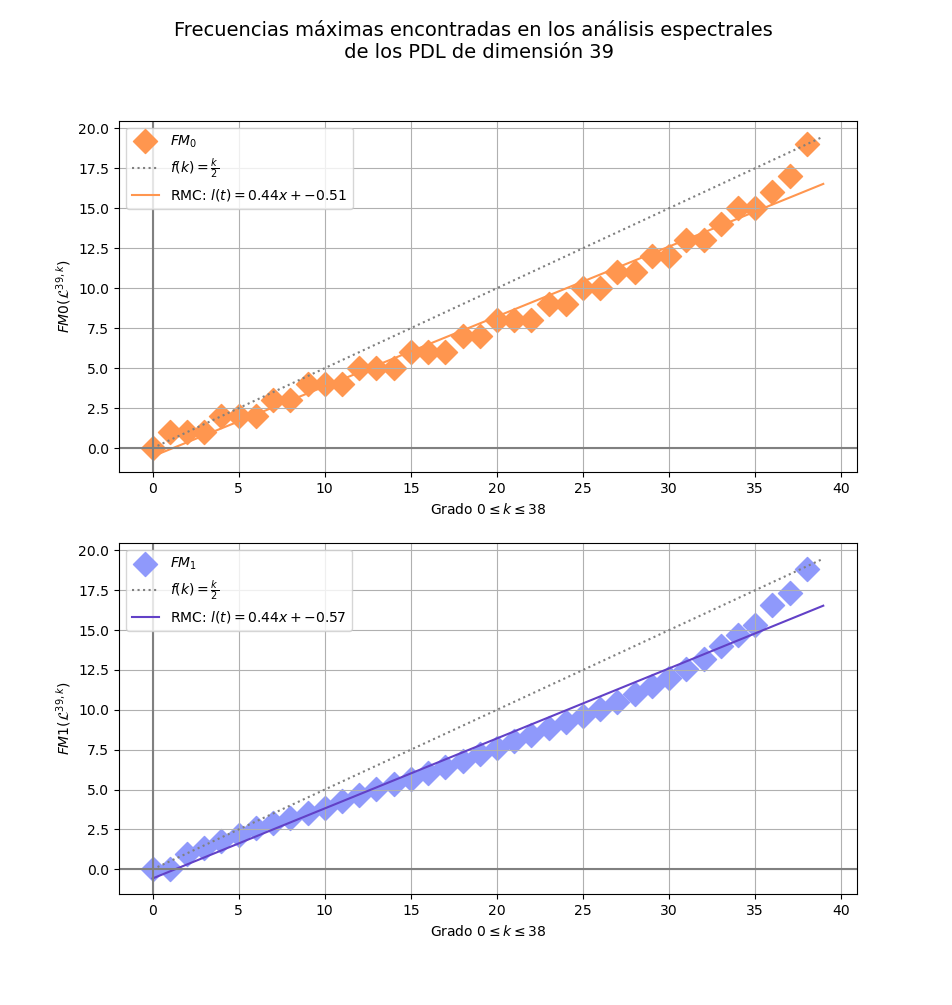
\includegraphics[scale = 0.6]{./estudios_espectrales/39} 
\end{figure}	

\begin{figure}[H]
	\sidecaption{
	\label{fig: 65}
	}
	\centering
	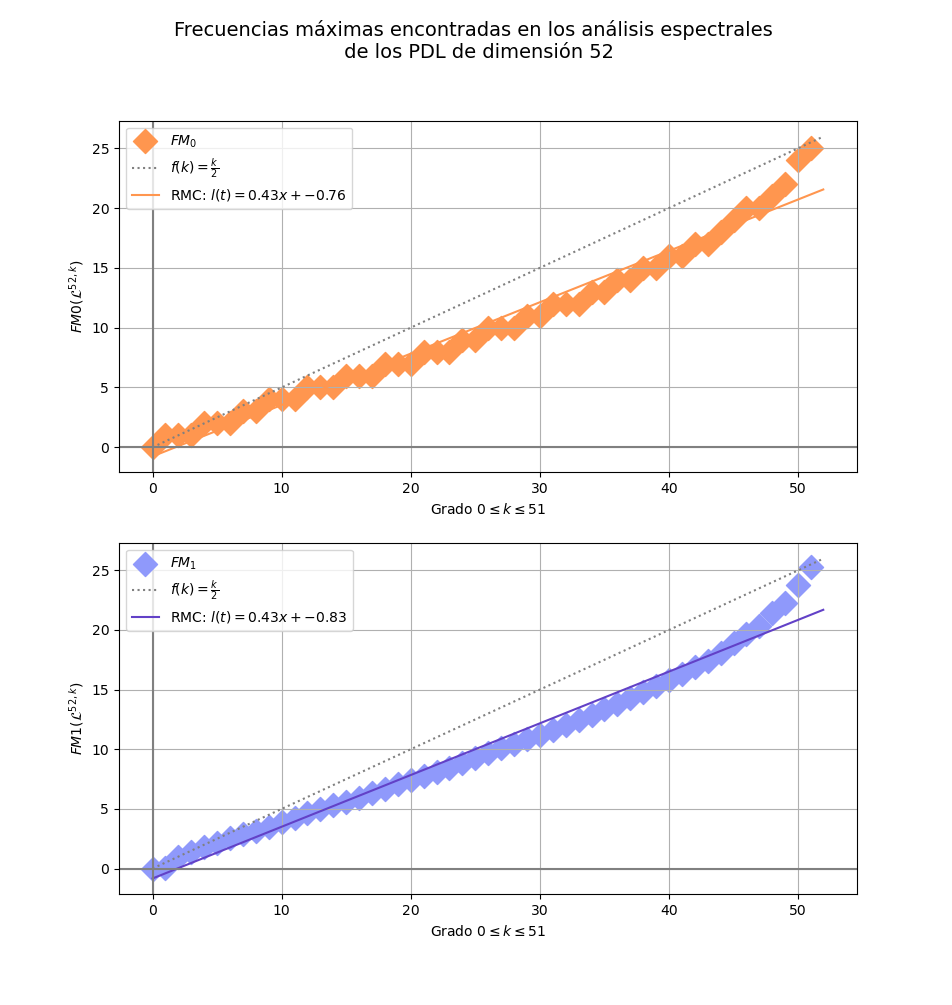
\includegraphics[scale = 0.6]{./estudios_espectrales/52} 
\end{figure}	

\begin{figure}[H]
	\sidecaption{
	Concluimos con la gráfica de las nubes de puntos
	de las que se habló en la figura 
	\ref{fig: ejemplo_pregunta3_1}.
	\label{fig: pendiente_oOrigen}
	}
	\centering
	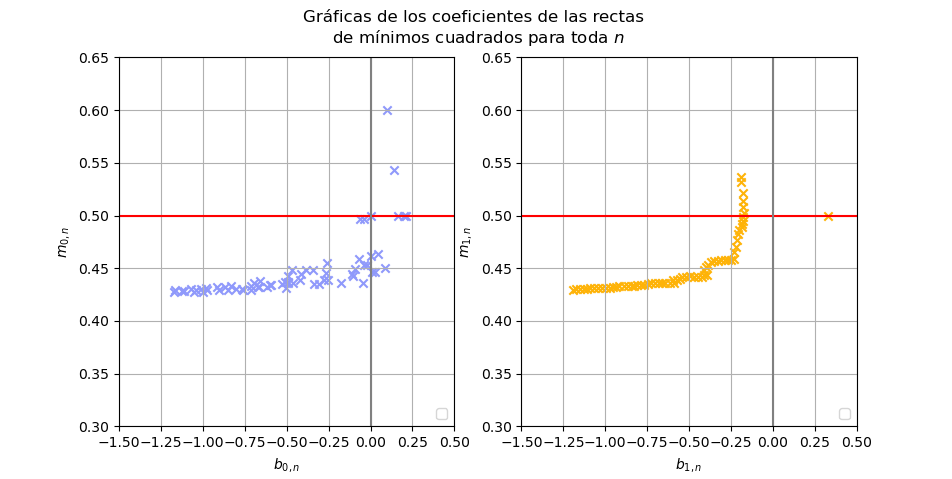
\includegraphics[scale = 0.6]{./estudios_espectrales/pendiente_oOrigen} 
\end{figure}	

\subsection{Sobre la frecuencia real de los PDL (cambia título)}

Para hacer nuestros análisis espectrales, hemos
usado la dimensión $n$ del PDL $\cali{L}^{n, k} \in \IR^{n}$
en cuestión
para buscar, en base a máximos globales
del espectro 
$\Sigma_{x}: [0, \frac{n}{2}] \longrightarrow [0,1]$, la
mejor frecuencia $\omega$ para aproximar la gráfica
de $\cali{L}^{n,k}$ en base a un sinusoide discreto
de dimensión $n$. \\


Note que en esa discusión nunca hablamos de 
parámetros importantes para, de forma canónica, hacer
un análisis espectral, como lo son la
duración en tiempo de la señal o la frecuencia
de muestreo.

\begin{defi}
\label{def: tiempo y frec de muestreo}
La cantidad de muestras tomadas (de forma uniforme)
de una señal por unidad de tiempo 
será denotada por $F_{s}$ y llamada \textbf{frecuencia
de muestreo} del análisis. A la cantidad de unidades de
tiempo que dura la medición se le denotará por $T$. \\

A la cantidad total de muestras tomadas se le denotará
por $L$.
\end{defi}

De las definiciones se sigue de inmediato que
\begin{equation}
\label{eq: relacion L, T Fs}
L = T F_{s}.
\end{equation}
\begin{figure}[H]
	\sidecaption{
	Adoptamos la convención de empezar a medir 
	un bloque de $F_{s}$ mediciones desde que inicia la
	unidad de tiempo (que, en el caso de la figura, se ha
	fijado como segundos).
	\label{fig: Fs 1}
	}
	\centering
	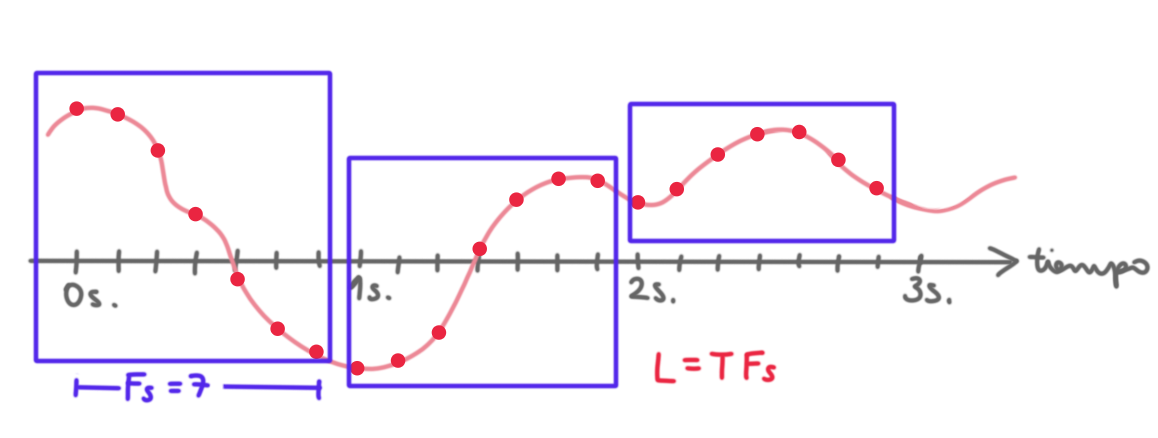
\includegraphics[scale = 1]{Fs_1} 
\end{figure}	

Nosotros, por el momento, sólo nos
hemos enfocado en buscar
una frecuencia $\omega \in [0, \frac{n}{2}]$ que de lugar
a un sinusoide que aproxime bien la gráfica
de $\cali{L}^{n,k}$;
observe que, al hacer esto, hemos supuesto de forma
implícita que estamos estudiando una señal
de duración una unidad de tiempo
($T = 1$) de longitud $n$
(o sea, $L = F_{s} = n$). \\
Supongamos ahora que
tenemos una señal $x$ que consta de $L$ mediciones, siendo
$F_{s}$ la frecuencia de muestreo.
\begin{figure}[H]
	\sidecaption{
	Para la imagen, hemos fijado $F_{s}= 10$
	y $L = 40$.
	\label{fig: frecuencia 1}
	}
	\centering
	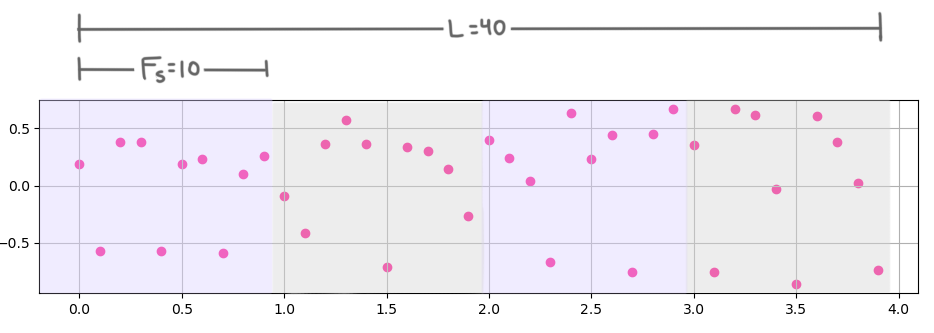
\includegraphics[scale = 0.45]{frecuencia_1} 
\end{figure}	

Sea ahora $2 \leq n \leq L$ y
supogamos que
se hizo el análisis
espectral 
de una sección $x_{|n}$ de tal señal
que conste de $n$ puntos
(usando el espectro
$\Sigma_{x}: [0, \frac{n}{2}]
\longrightarrow [0,1]$).
Digamos que, como conclusión de ese análisis, se
obtuvo que un sinusoide de frecuencia $\omega \in [0, \frac{n}{2}]$
ajusta bien \textit{esa sección particular 
$x_{|n}$
de la señal $x$}.
\begin{figure}[H]
	\sidecaption{
	Para la imagen, hemos fijado $n= 6$;
	se calculó que la mejor frecuencia para ajustar 
	los primeros $6$ puntos que componen la señal
	original $x$ es $w = 2$.
	\label{fig: frecuencia 2}
	}
	\centering
	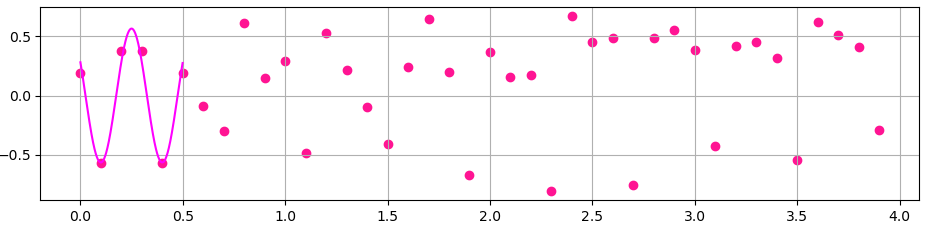
\includegraphics[scale = 0.45]{frecuencia_2} 
\end{figure}	

Observe que, en general, si se quisiera usar
directamente una frecuencia de $w$ para ajustar
a la señal $x$, la aproximación lograda en los
$n$ puntos escogidos previamente puede no ser válida.
\begin{figure}[H]
	\sidecaption{
	Usando los datos de la figura \ref{fig: frecuencia 2}, podriamos
	intentar en un principio usar a un sinusoide de frecuencia $2$
	para intentar modelar a la señal, pero un sinusoide de tal frecuencia,
	como es el caso de esta figura, puede que ni siquiera sea adecuado
	para modelar el pedazo $x_{|n}$ original a partir del cual se obtuvo
	la frecuencia $\omega$.
	\label{fig: frecuencia 2}
	}
	\centering
	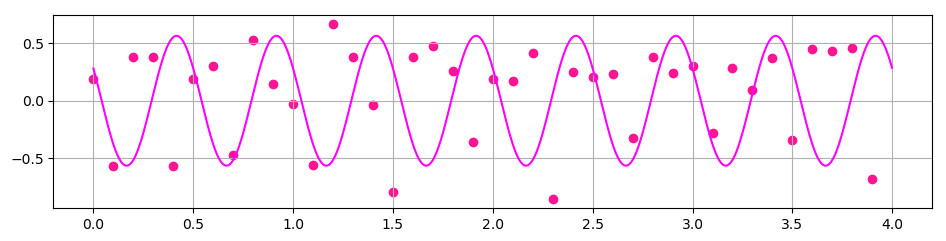
\includegraphics[scale = 0.45]{frecuencia_3} 
\end{figure}
Esto se debe a que	
tal frecuencia $\omega$ es buena para aproximar
a dichos $n$ puntos cuando se ha tomado como
unidad de tiempo a $n$, pero, 
por la forma en que fue muestreada la señal original $x$,
son $F_{s}$ (y no necesariamente $n$) la cantidad de puntos
que conforman una unidad. Así, puesto que con $\omega$
ciclos de un sinusoide se aproximaron $n$ puntos, 
la frecuencia que debe escogerse para aproximar a todos los $L$
puntos es
\begin{equation}
\label{eq: rel frecuencia real y ficticia}
\tilde{w} := \frac{F_{s}}{n} \omega.
\end{equation}

\begin{figure}[H]
	\sidecaption{
	Es con una simple regla de tres que se deduce
	la relación \eqref{eq: rel frecuencia real y ficticia}.
	\label{fig: frecuencia real}
	}
	\centering
	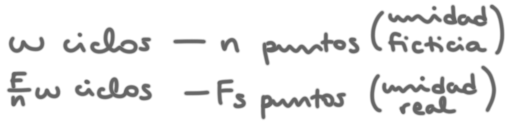
\includegraphics[scale = 1.4]{frecuencia_real} 
\end{figure}	
\begin{figure}[H]
	\sidecaption{
	Según los datos de las figuras
	\ref{fig: frecuencia 1}
	y \ref{fig: frecuencia 2}, con un sinusoide de frecuencia
	$\tilde{\omega} = 10/3$ se aproximan bien a los seis
	puntos en base a los cuales se encontró a la primera
	frecuencia $\omega$.
	\label{fig: frecuencia 4}
	}
	\centering
	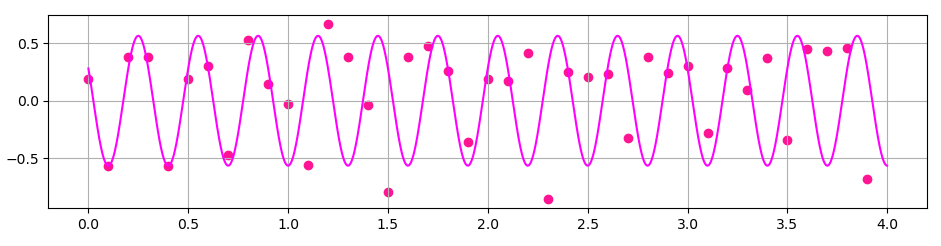
\includegraphics[scale = 0.45]{frecuencia_4} 
\end{figure}